\documentclass[10pt]{beamer}
% \documentclass[reqno]{beamer}

\usepackage{times}
\usepackage[utf8]{inputenc}  % pour les accents
\usepackage{euler}
\usepackage{amsmath}
\usepackage{amssymb}
\usepackage{dsfont}
\usepackage{amsthm}
\usepackage{color}
\usepackage{listings}
\usepackage{algorithm}
\usepackage{algorithmic}
\usepackage{booktabs}       % professional-quality tables
\usepackage{tikz}
\usetikzlibrary{decorations.pathreplacing}

%\newtheorem{algorithm}{Algorithm}

\newcommand\independent{\protect\mathpalette{\protect\independenT}{\perp}}
\def\independenT#1#2{\mathrel{\rlap{$#1#2$}\mkern2mu{#1#2}}} 

\newcommand{\ie}{\emph{i.e.}{}}
\newcommand{\st}{\text{\emph{s.t.}}{}}
\newcommand{\eg}{\emph{e.g.}{}}
\newcommand\iid{\ensuremath{\mathit{i.i.d.}}\ }
\newcommand{\rv}{\emph{r.v.}{}}
\newcommand{\ud}{\text{d}{}}
\newcommand{\ind}{\mathds{1}{}}

\newcommand\red{\color{red} }
\newcommand\blue{\color{blue} }
\newcommand{\crit}{\mathcal{C}}

\definecolor{blue}{rgb}{0.1,0.1,0.65}
\definecolor{red}{rgb}{0.7,0.1,0.1}

\def\argmin{\operatornamewithlimits{arg\,min}}
\def\argmax{\operatornamewithlimits{arg\,max}}
\def\supess{\operatornamewithlimits{ess\,sup}}

% \DeclareMathOperator{\argmin}{argmin}
\def\bb{\mathbb}
\def\mb{\mathbf}
\def\leb{\text{Leb}}


% \usetheme{Darmstadt} %\theme
% \useoutertheme{sidebar}
% \useinnertheme{circles}

%\usecolortheme{beaver}
%\usecolortheme{seagull}
\usecolortheme{seahorse}
%\setbeamercolor*{frametitle}{parent=palette primary}


% \useoutertheme{infolines}
% \setbeamertemplate{navigation symbols}{} 
% \setbeamertemplate{footline}{
%   \hspace*{.5cm}\tiny{%\insertauthor
%     \hspace*{50pt}
%     \hfill\insertframenumber%/\inserttotalframenumber
%     \hspace*{.5cm}}\vspace*{.1cm}} 

%\addtobeamertemplate{footline}{\insertframenumber/\inserttotalframenumber} 
% \setbeamertemplate{footline}{\hspace*{.5cm}\scriptsize{%\insertauthor
%     \hspace*{50pt} \hfill\insertframenumber\hspace*{.5cm}}\vspace*{.1cm}} 

%\setbeamertemplate{theorems}[numbered]

 \setbeamercolor{block title}{bg=blue!3,fg=blue}
 \setbeamercolor{block body}{bg=blue!3,fg=black}

% %\setbeamercolor{block title alerted}{bg=green!10,fg=black}
% \setbeamercolor{block body alerted}{bg=red!10,fg=black}

% \setbeamercolor{block title example}{bg=green!10,fg=black}
% \setbeamercolor{block body example}{bg=green!10,fg=black}


\title{
Machine Learning Methods for Anomaly Detection
}

\author[Nicolas Goix]{ Nicolas Goix \\
% \\
% \vspace{1em}
 {\tiny LTCI, CNRS, Telecom ParisTech, Université Paris-Saclay, France 
 }
}
%}
\date{PhD Defence, Telecom Paristech, October 2016}



\AtBeginSubsection[]
{
 \begin{frame}<beamer>
 \frametitle{}
 \tableofcontents[currentsection,currentsubsection]
 \end{frame}
}

\begin{document}
\begin{frame}
 \titlepage
\end{frame}


% \begin{frame}
% \frametitle{Outline}
% \tableofcontents%[section, subsection]
% \end{frame}

% \begin{frame}
%   \frametitle{Outline}
%   \tableofcontents
% \end{frame}


%\section{Introduction}



\begin{frame}
\frametitle{Anomaly Detection (AD)}

\textbf{`Finding patterns in the data that do not conform to expected behavior'}
\begin{figure}
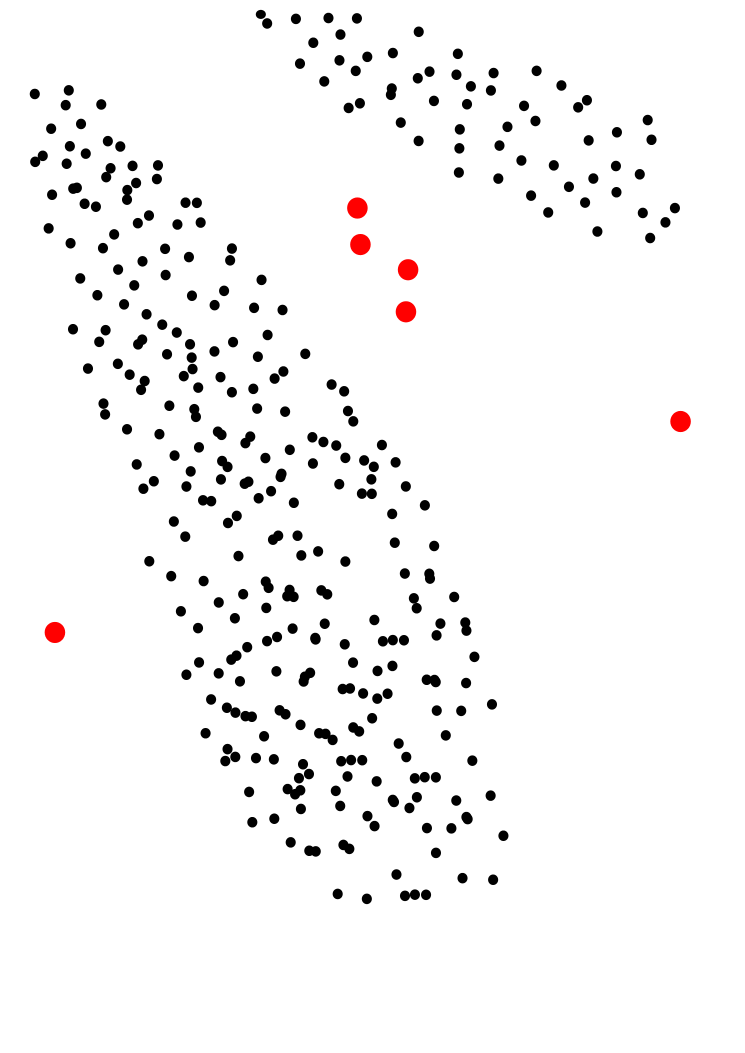
\includegraphics[height=5cm]{AD_intro.png}
\end{figure}
Huge number of applications: Network intrusions, credit card fraud detection, insurance, finance, military surveillance,... \\~\\
\end{frame}



\begin{frame}
\frametitle{Machine Learning context}
%In a machine learning context, AD can been seen as a classification task but where the usual assumption -dataset contains info regarding all classes- breaks down.
\begin{block}{Different kind of Anomaly Detection}
\begin{itemize}
\item \textbf{Supervised} AD {\red (not dealt with)}\\
Labels available for both normal data and anomalies\\
(similar to rare class mining)\\~\\

\item \textbf{Novelty Detection} {\red (our theoretical framework)}\\
The algorithm learns on normal data only\\~\\

\item \textbf{Outlier Detection} {\red (extended application framework)}\\
Training set (unlabeled) = normal + abnormal data \\
(assumption: anomalies are very rare)
\end{itemize}
\end{block}
\end{frame}


\begin{frame}
\frametitle{Outlines}
%In a machine learning context, AD can been seen as a classification task but where the usual assumption -dataset contains info regarding all classes- breaks down.
An AD algorithm returns a {\blue scoring function $s: \mathbb{R}^d \to \mathbb{R}$}.\\
It represents the {\blue `degree of abnormality'} of an observation $x \in \mathbb{R}^d$ \\~\\

\begin{block}{}
\begin{itemize}
\item Part I: Performance criterion on {\blue $s$}.\\
{\footnotesize ~~(model selection)} \\~\\~\\
%{\small ~~~~~~~~~~~~ $\to$ Evaluation criterion for AD algorithms.}\\~\\~\\~\\
\item Part II: Building good {\blue $s$} on extreme regions. \\
{\footnotesize ~~ (model design)}
%{\small ~~~~~~~~~~~~ $\to$ Gaining in accuracy on extreme regions.}
\end{itemize}
\end{block}
\end{frame}

\section{Part I: performance criterion}
\subsection{Definition}

\begin{frame}
\frametitle{(unsupervised) performance criterion}

%\subsection{Goal of Anomaly Detection }
%Anomaly: "an observation which deviates so much from other observations as to arouse suspicions that it was generated by a different mechanism (Hawkins 1980)"

\begin{block}{Such a criterion allows:}
\begin{itemize}
\item{1-} To build good {\blue $s$} by optimizing this criterion.
\item{2-} To evaluate any AD algorithm without using any labels.
\end{itemize}
\end{block}

\begin{block}{Practical motivations:}
Most of the time, data come without any label.\\
{\footnotesize ~~~~~~ $\to$ no ROC or PR curves!}
\end{block}

\begin{block}{Idea:}
\centering
How good is an anomaly detection algorithm?
$$\downarrow$$
How good is it estimating the level sets?
\end{block}
\end{frame}



\begin{frame}
\frametitle{Context}
%In a machine learning context, AD can been seen as a classification task but where the usual assumption -dataset contains info regarding all classes- breaks down.

\begin{block}{Novelty Detection { \footnotesize (`One-Class Classification', `semi-supervised AD')}}~\\~\\

\begin{itemize}
\item \textbf{Data: {\red inliers}}.\\
i.i.d. observations in $\mathbb{R}^d$ from the normal behavior, density {\red $f$}.\\~\\
%{\footnotesize Remark: In practice, data can be polluted by a small proportion of anomalies.}

\item \textbf{Output to evaluate: {\blue scoring function $s: \mathbb{R}^d \to \mathbb{R}$}} \\
%{\footnotesize
%- AD algorithms return {\blue $s: \mathbb{R}^d \to \mathbb{R}$}.\\
- $s$ defines a {\blue pre-order} on $\mathbb{R}^d$ = `degree of abnormality'.\\
- $s$ level sets are estimates of $f$ level sets.\\
- $s$ can be interpreted as a box which contains {\blue an infinite number of level sets estimates} (at different levels).\\~\\
\end{itemize}

\textbf{Remark.} Perfect scoring functions: $s=f$ or $s=2f+3$ or $s=T \circ f$ any increasing transform of $f$. \\
%($f=2s$, $f=s^2$ if $s \ge 0$, ...).

\end{block}
\end{frame}


\begin{frame}
\frametitle{Problem reformulation}
We want a criterion $\mathcal{C}(s)$ which measures \emph{how well the level sets of $f$ are approximated by those of $s$}.
%$$\mathcal{C}(s) (t) \simeq ~\inf_{u>0}~ \leb(\{ s >u\}~\Delta~\{f>t\})$$
\begin{block}{}
\begin{itemize}
\item \textbf{Fact:} For any strictly increasing transform $T$, level sets of $T \circ f$ are exactly those of $f$.\\
$\Rightarrow$ Criterion $\mathcal{C}(s) = \|s-f\|$ is not relevant! ($s = 2f$ is perfect)\\~\\

\item \textbf{We are looking for a criterion s.t:}\\
- $\crit^{\Phi}(s) = \| \Phi(s) - \Phi(f) \|$ with $\Phi$ s.t. $\Phi(T \circ s) = \Phi(s)$. \\
- $ \{ \text{level sets of optimal }~ s^*\} = \{ \text{level sets of } ~f \}$. \\
- $\crit^{\Phi}(s)$ = `distance' between level sets of $s$ and those of $f$.

\end{itemize}
\end{block}
 $\Rightarrow \Phi(s) := MV_s$ or $EM_s$, the Mass-Volume and Excess-Mass curves of $s$.
\end{frame}


\begin{frame}
\frametitle{Criteria satisfying these requirements: MV and EM}

\begin{block}{Mass-volume and excess-mass curves}
\begin{itemize}
% \footnotesize{
\item \textbf{Definitions:}
\begin{align*}
& MV_s(\alpha) ~=~ \inf_{\Omega \text{ level-set of } s}~~~ \big\{\leb(\Omega) ~~~~s.t.~~~~ \mathbb{P}(\mb X \in \Omega) \ge \alpha\big\} \\
& EM_s(t) ~~=~ \sup_{\Omega \text{ level-set of } s}~~~\big\{ \mathbb{P}(\mb X \in \Omega) ~-~ t \leb(\Omega) \big\}
\end{align*}


% \footnotesize{
\item \textbf{Optimal curves:}
\begin{align*}
&MV^*(\alpha) ~=~ \min_{\Omega~ \text{borelian}} ~\big\{\leb(\Omega) ~~~\st~~ \mathbb{P}(\mb X \in \Omega) \ge \alpha\big\}\\
&~~~~~~~~~~~~~~~~~~~~~~~~~~~~~~~~~~~~~~~~~~~~~~~~~~~~~~~~~~~~~= MV_f(\alpha) = MV_{T \circ f}(\alpha)\\~\\
&EM^*(t) ~~=~ \max_{\Omega\text{ borelian} } ~\big\{{\mathbb{P}} (\mb X\in \Omega)-t\leb(\Omega) \big\}\\
&~~~~~~~~~~~~~~~~~~~~~~~~~~~~~~~~~~~~~~~~~~~~~~~~~~~~~~~~~~~~~= EM_f(t) = EM_{T \circ f}(t)
\end{align*}

\end{itemize}
\end{block}
\end{frame}


\begin{frame}
\frametitle{MV and EM criteria}
\begin{itemize}
\item \textbf{Interpretation:} $(EM_s - EM_f)(t) \simeq ~\inf_{u>0}~ \leb(\{ s >u\}~\Delta~\{f>t\})$ \\~\\~\\
% \begin{align*}
% &\| EM_s - EM_f\|_{L^1(I)} : \text{ how well $t$-level sets of $f$ are approximated by}\\
% &~~~~~~~~~~~~~~~~~~~~~~~~~~~~~~~~~~\text{ level sets of $s$, $t \in I$}.\\
% &\| MV_s - MV_f\|_{L^1(J)} : \text{ how well $\alpha$-level sets of $f$ are approximated by} \\
% &~~~~~~~~~~~~~~~~~~~~~~~~~~~~~~~~~~\text{ level sets of $s$, $\alpha \in J$}.\\
% %&(EM_s - EM_f)(t) \simeq \inf_{u>0} Leb (\{ s >u\}\Delta\{f>t\})
% \end{align*}


\item How well {\red $t$}-level sets of $f$ are approximated by level sets of $s$, ${\red t} \in I$ ? \\
{\centering $\downarrow$\\~\\
how {\blue small} is $EM_s - EM_f$ on $I$ ? ~~$\Leftrightarrow$~~ how {\blue large} is $EM_s$ on $I$ ?\\~\\~\\~\\}

\item How well {\red $\alpha$}-level sets of $f$ are approximated by level sets of $s$, ${\red \alpha} \in J$ ? \\
{\centering $\downarrow$\\~\\
 how {\blue small} is $MV_s - MV_f$ on $J$ ? ~~$\Leftrightarrow$~~  how {\blue small} is $MV_s$ on $J$ ?\\}
 
\end{itemize}


\end{frame}

\begin{frame}
\begin{figure}
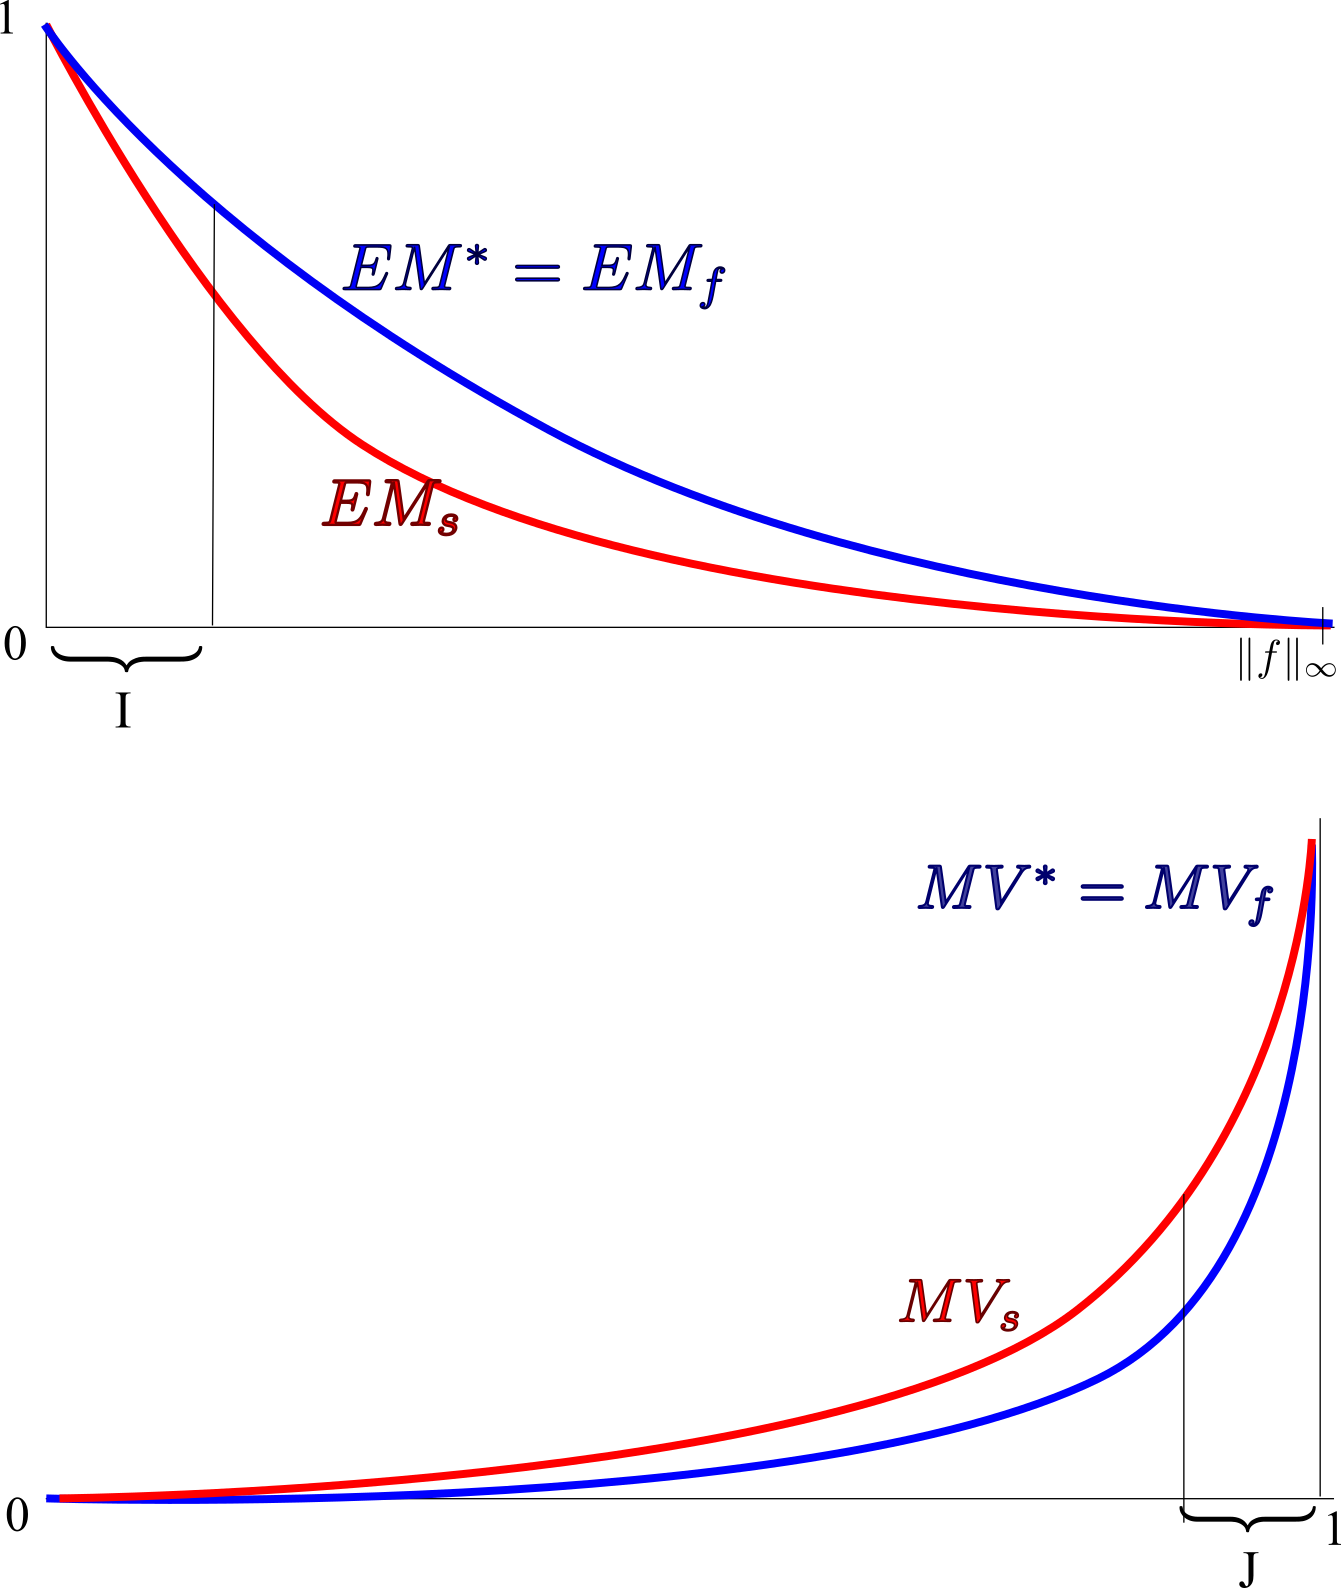
\includegraphics[width = 0.7\linewidth]{emmv.png}
\end{figure}
\end{frame}

\subsection{Learning a scoring function}

\begin{frame}
\frametitle{Learning a scoring function with M-estimation}



We are looking for nearly optimal scoring functions of the form {\blue $s = \sum_{j=1}^N a_j \mathds{1}_{x \in \Omega_j}$}, with $a_j \ge 0$,~ $\Omega_j \in \mathcal{G}$.\\~\\


\begin{block}{}
{\blue Procedure}:  For $k=1, \ldots, N$,
%
\begin{align*}
&\widehat \Omega_{t_{k+1}} =~~ \argmax_{\Omega \supset \widehat \Omega_{t_k}} ~~~~ \mathbb{P}_n(X \in \Omega) ~-~ t_{k+1} \leb(\Omega)\\
&t_{k+1} ~~=~ \frac{t_k}{(1 + \frac{1}{\sqrt n})}
\end{align*}
%
%where $\mathbb{P}_n(X \in \Omega) = \frac{1}{n} \sum_{i=1}^n \mathds{1}_{X_i \in \Omega}$, we obtain
$s_N(x) := \sum_{j=1}^N(t_j - t_{j+1}) \mathds{1}_{x \in \Omega_{t_j}}$
\begin{figure}
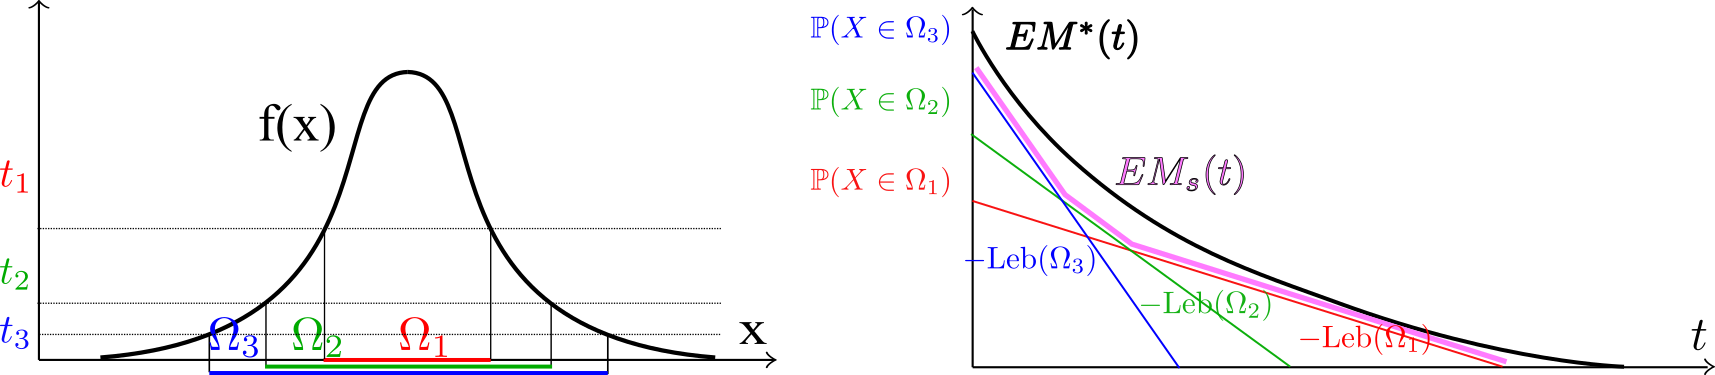
\includegraphics[width=\linewidth]{em_optim.png}
\end{figure}
\end{block}

\end{frame}

\begin{frame}
\frametitle{Learning a scoring function with M-estimation}

\begin{block}{}
{\blue Rates}: (if density bounded and without flat parts, $\mathcal{G}$ VC-class)
\begin{align*}
\sup_{t \in ]0,t_1]}|EM^*(t)-EM_{s_N}(t)| ~\le~ \left[A+\sqrt{2\log(1/\delta)}\right]\frac{1}{\sqrt n}+ bias(\mathcal{G}) + o_N(1)
\end{align*}
\end{block}
~\\~\\~\\~\\~\\~\\
\begin{figure}
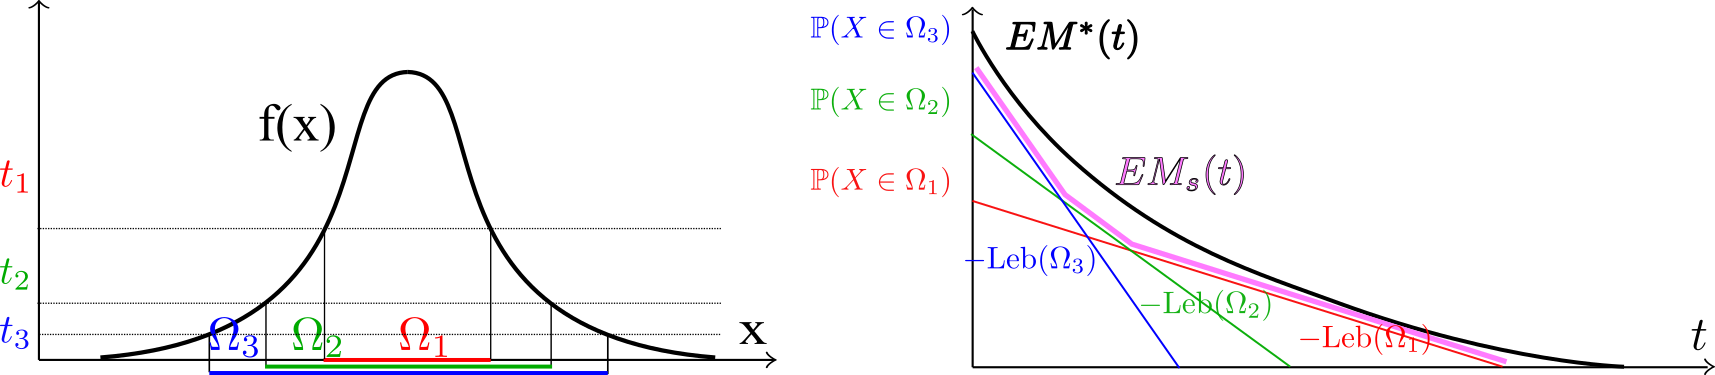
\includegraphics[width=\linewidth]{em_optim.png}
\end{figure}

\end{frame}


\subsection{Evaluating a scoring function}


\begin{frame}
\frametitle{Evaluation of scoring functions}

\begin{itemize}
\item \textbf{Estimation:}
\small{
\begin{align*}
&\widehat{MV}_s(\alpha) = \inf_{u \ge 0} ~~~\leb(s \ge u) ~~~~\st~~~~ \mathbb{P}_n(s \ge u) \ge \alpha\\
&\widehat{EM}_s(t) = \sup_{u \ge 0} ~~~\mathbb{P}_n(s \ge u) ~-~ t \leb(s \ge u)
\end{align*}
}

\item \textbf{Empirical criteria:}
\small{
\begin{align*}
\widehat{\crit}^{EM}(s) &= \| \widehat{EM}_s \|_{L^1(I)}  &&I = [0,\widehat{EM}^{-1}(0.9)],\\
\widehat{\crit}^{MV}(s) &= \| \widehat{MV}_s \|_{L^1(J)}  &&J = [0.9, 1],
\end{align*}
}


\item \textbf{Issue:}
\small{
The volume $\leb(s \ge u)$ has to be estimated (Monte-Carlo). Challenging in large dimensions.
}

\end{itemize}
\end{frame}




\begin{frame}
\frametitle{Evaluation: Heuristic solution}

\begin{block}{Feature sub-sampling (random projection) and averaging}~\\

\small{
%\begin{algorithm}
\begin{algorithmic}

  \STATE \textbf{Inputs}: AD algorithm $\mathcal{A}$, data set $X$ size $n \times d $, feature sub-sampling size $d'$, number of draws $m$.\\~\\
  \FOR{$k=1,\ldots,m$}
    \STATE{-randomly select a sub-group $F_k$ of $d'$ features}
    \STATE{-compute the associated scoring function $s_{k} = \mathcal{A}\big((x^j_i)_{1 \le i \le n,~j \in F_k}\big)$}
    \STATE -compute $\widehat{\crit}_k^{EM} = \| \widehat{EM}_{s_k} \|_{L^1(I)}$  or $\widehat{\crit}_k^{MV} = \| \widehat{MV}_{s_k} \|_{L^1(J)}$
  \ENDFOR \\~\\

  \STATE \textbf{Return} performance criteria: $$\widehat{\crit}^{EM}_{high\_dim} (\mathcal{A})= \frac{1}{m} \sum_{k=1}^m\widehat \crit_k^{EM} \text{~~~~or~~~~} \widehat{\crit}^{MV}_{high\_dim}(\mathcal{A}) = \frac{1}{m} \sum_{k=1}^m\widehat \crit_k^{MV}~.$$

\end{algorithmic}
%\end{algorithm}
}

\end{block}
\end{frame}


\section{Part II: Learning accurate scoring functions on extreme regions}









\subsection{Multivariate EVT \& Representation of Extremes}

\begin{frame}
\begin{alertblock}{General idea of our work}
\begin{itemize}
\item Extreme observations play a special role when dealing with outlying data.\\~\\
\item But no algorithm has \textbf{specific treatment for such multivariate extreme observations}.\\~\\
\item Our goal: Provide a method which can improve performance of standard AD algorithms by combining them with a \textbf{multivariate extreme analysis} of the \textbf{dependence structure}.\\~\\
\end{itemize}
\end{alertblock}
\end{frame}

\begin{frame}
\begin{figure}
\centering
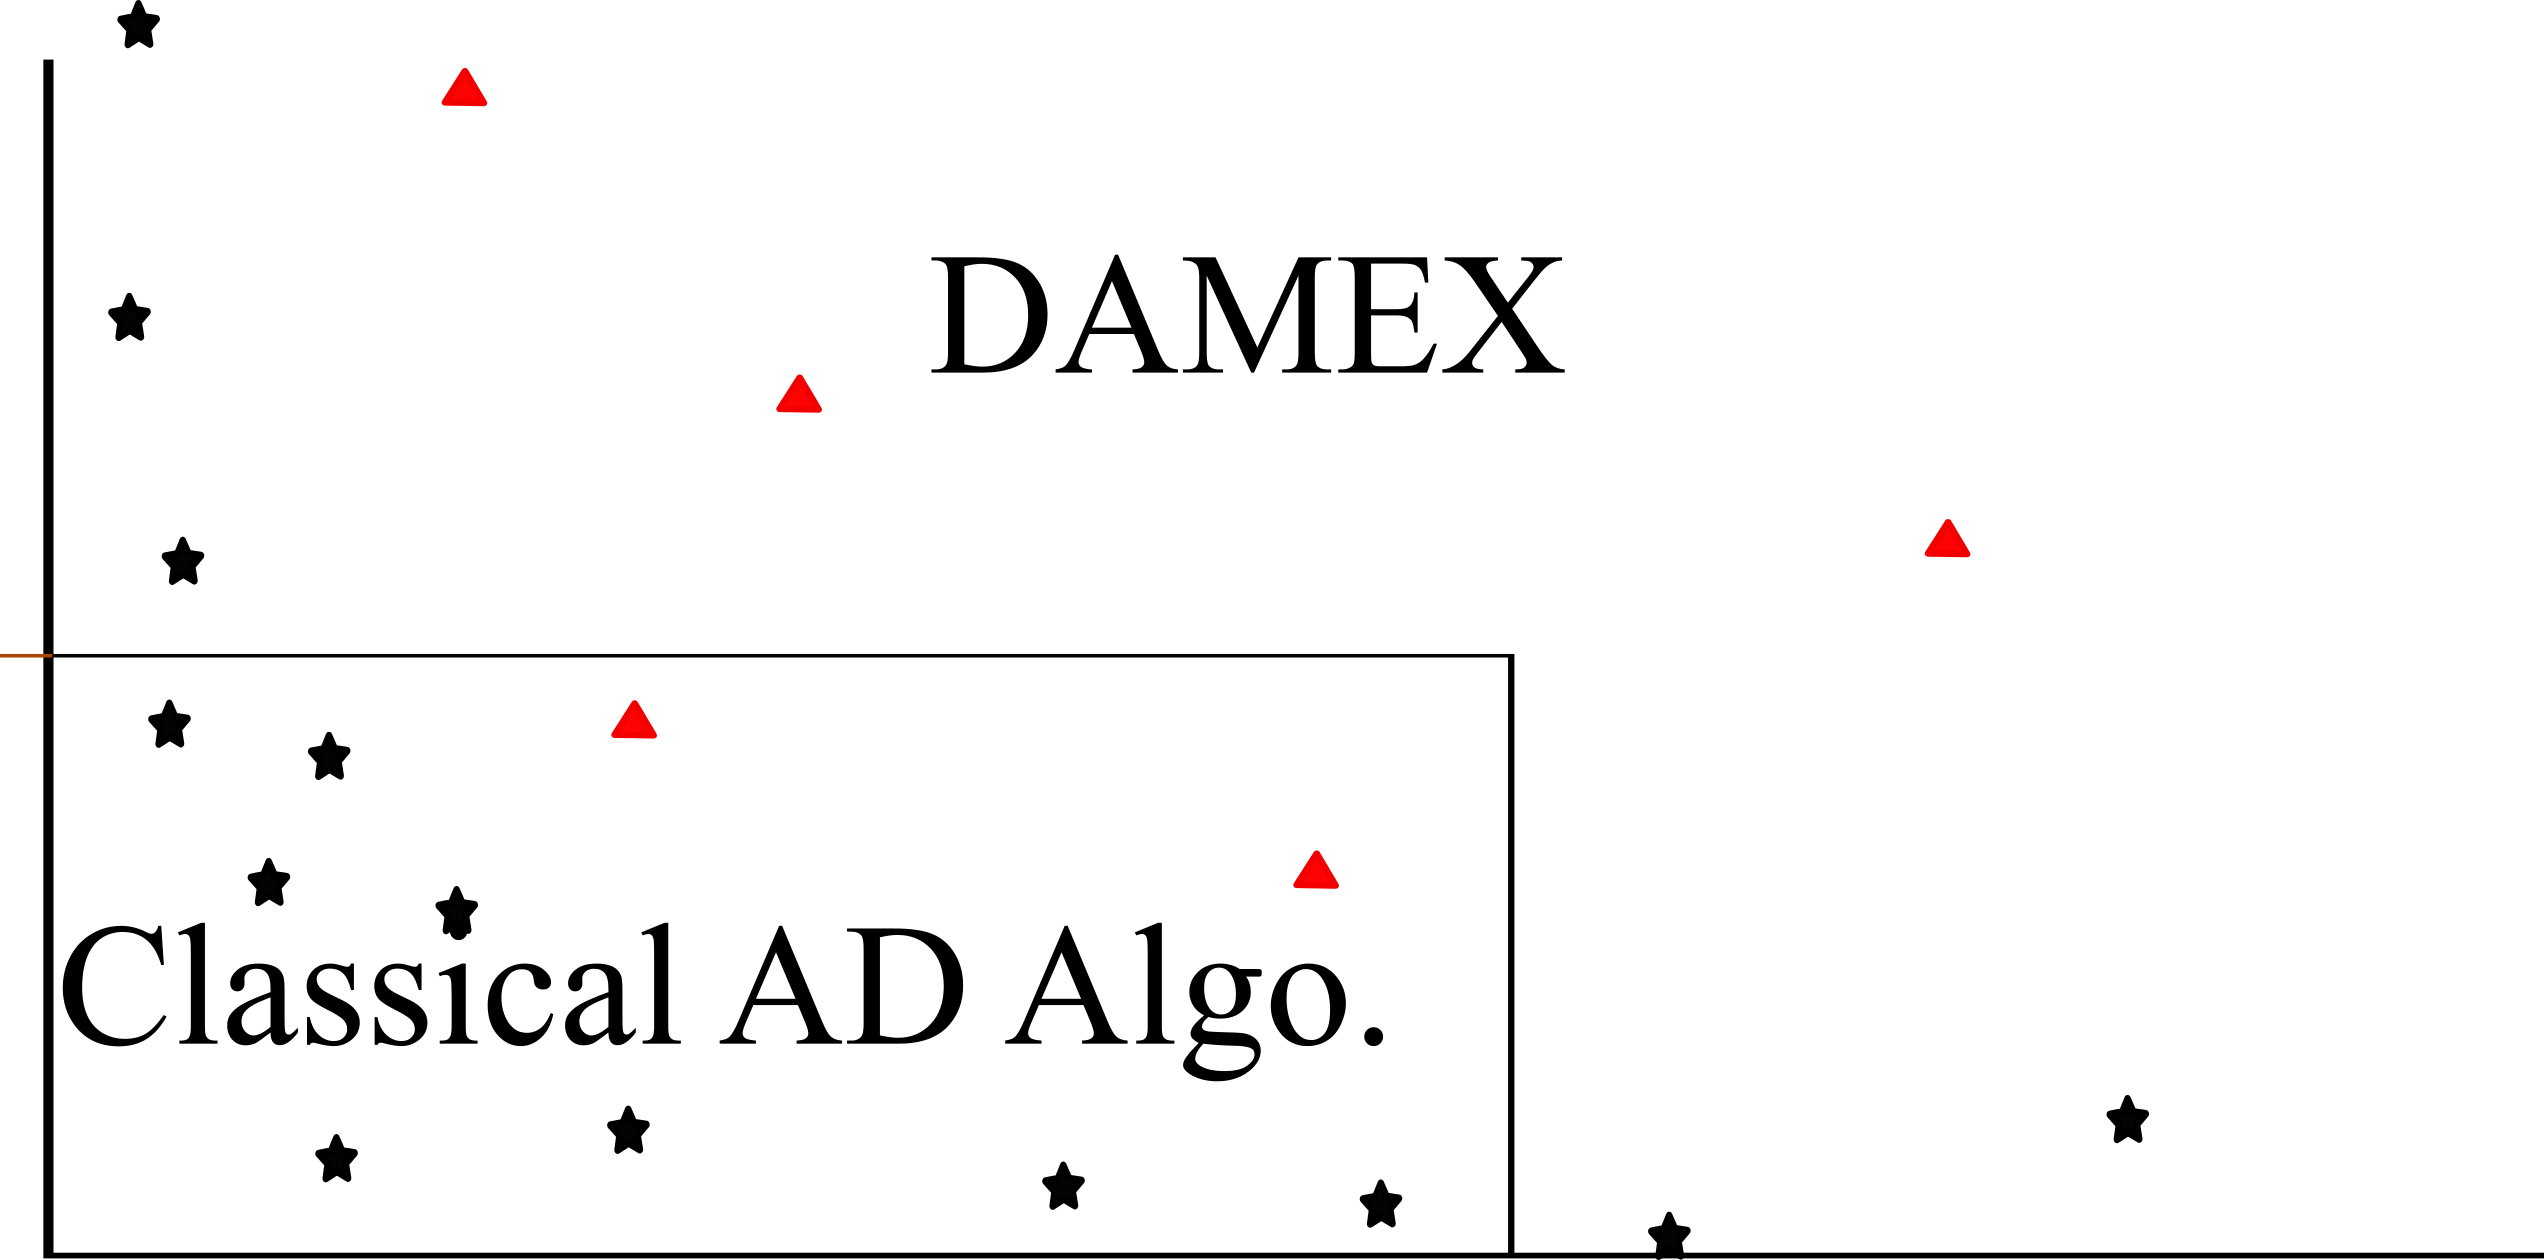
\includegraphics[height=3.5cm]{sourcefigs/extreme_AD.png}
\end{figure}
\end{frame}


\begin{frame}
\centering
{\LARGE Goal:}\\
\begin{align*}
\mb X = (X_1,\ldots,X_d)
\end{align*}
{\Large Find the groups of features which can be large together}
\begin{align*}
\text{ex:~~~~}\{X_1, X_2\},~\{X_3, X_6, X_7\},~\{X_2,X_4,X_{10},X_{11}\}
\end{align*}
~\\~\\
$\Leftrightarrow$ \Large{Characterize the extreme dependence structure}\\~\\~\\

Anomalies~~=~~ points which violate this structure

\end{frame}



\begin{frame}
\frametitle{Framework}
\begin{itemize}
\item \textbf{Context} 

  \begin{itemize}
  \item Random vector    $  \mb X = (X_{1},\ldots,X_{d})  $
    \vspace{0.3cm}
  \item Margins: $X_{j}\sim F_j$ ~~~~~~~~~($F_j$ continuous)\\
    \vspace{0.3cm}
  \end{itemize}
    \vspace{0.3cm}

\item \textbf{Preliminary step: Standardization of each marginal}\\
    \vspace{0.3cm}
    \begin{itemize}
    \item   Standard Pareto: 
    $V_{j} = \frac{1}{1- F_j (X_{j})} $  ~~~~\Big($\mathbb{P}(V_j \ge x) = \frac{1}{x}$,~~ $x\ge 1$\Big) \\
    \end{itemize}
% OR\\
%     \vspace{0.3cm}

%   \item Uniform:
%     $U_{j} = 1- F_j (X_{j}) $
%     \vspace{0.3cm}


\end{itemize}

\end{frame}


\begin{frame}
\frametitle{Problematic}
\vspace{0.2cm}
Joint extremes: $\mb V$'s distribution above large thresholds? 
\vspace{0.2cm}
    $$
    \mathbb{P}(\mb V\in A) \text{?} ~~~~ (A  \text{ `far from the origin'}).
    $$
  \begin{figure}
    \centering
    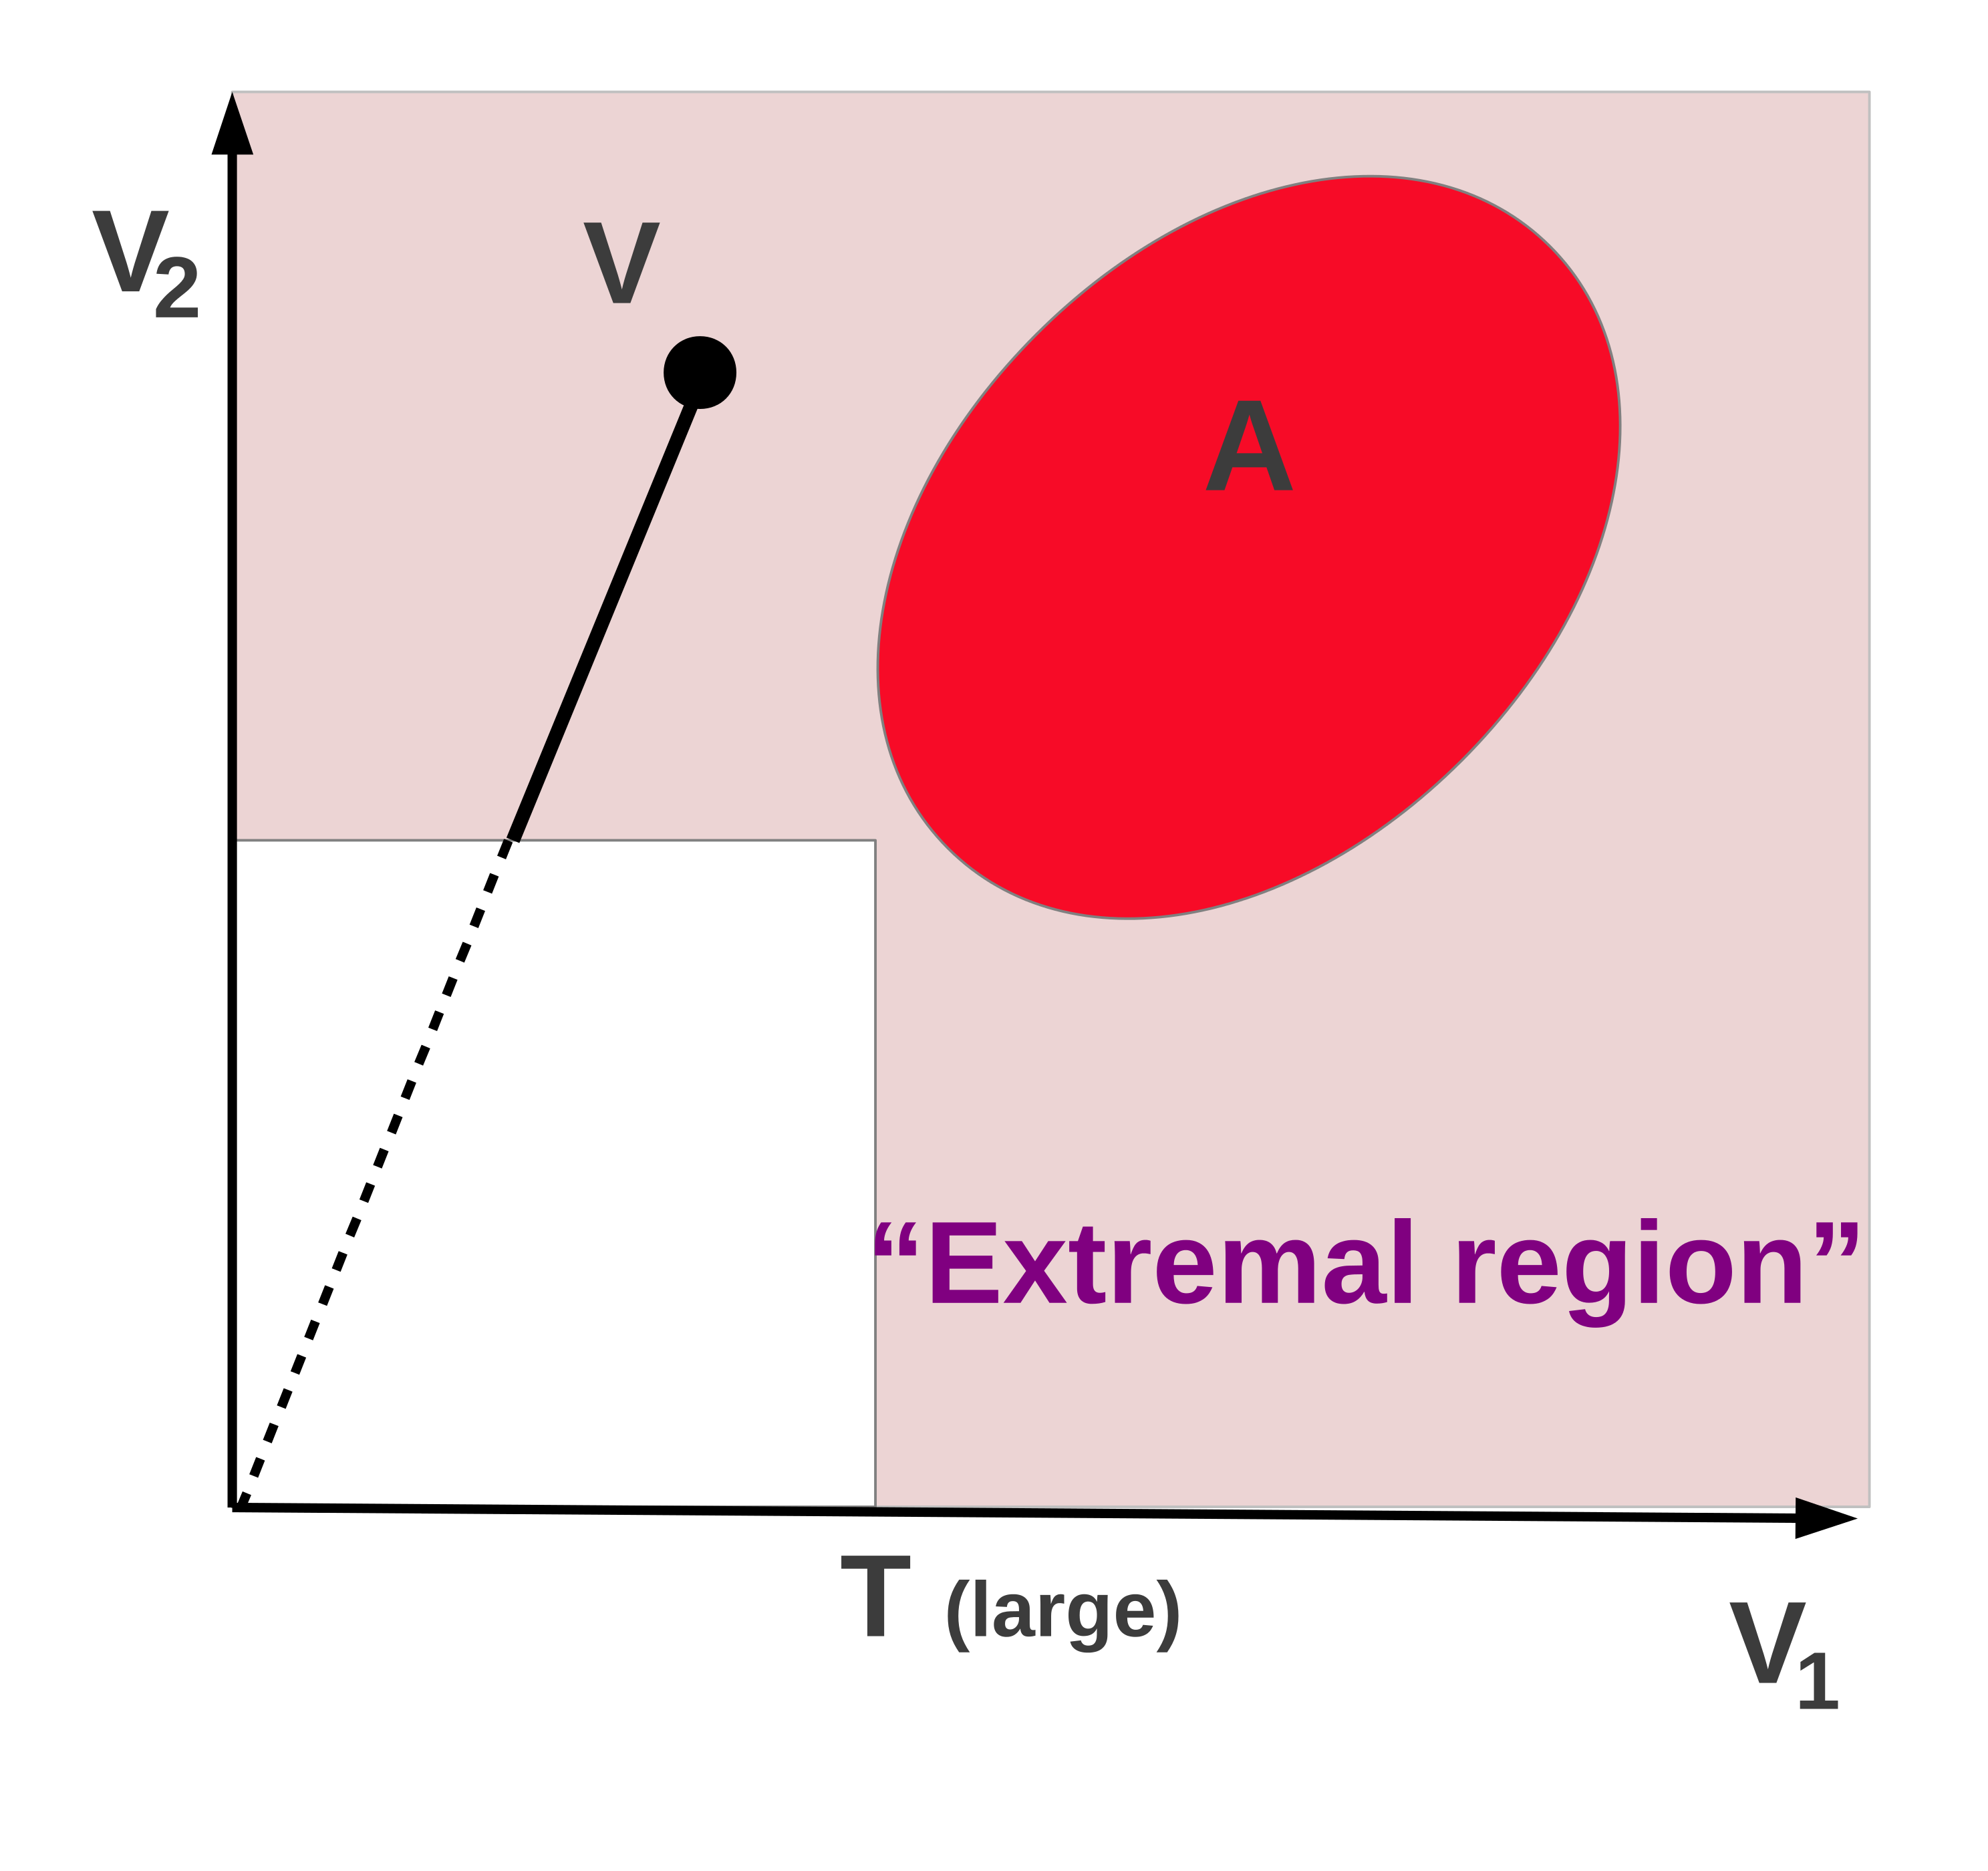
\includegraphics[scale=0.3]{sourcefigs/application4.png}
  \end{figure}
\end{frame}

\begin{frame}
  \frametitle{Fundamental hypothesis and consequences}%, fundamental result}

  \begin{itemize}
\item Standard assumption: let $A$ extreme region, $$\mathbb{P}[\mb V\in t~A] \simeq t^{-1}\mathbb{P}[\mb V\in A] \quad \text{(radial homogeneity)} $$ 
\item Formally,
\begin{exampleblock}{\textbf{regular variation} (after standardization):}
 $0 \notin \overline A$ $$ t \mathbb{P}[\mb V\in t~A]\xrightarrow[t\to\infty]{}
 \mu(A),\qquad\mu:\text{ exponent measure} $$
\end{exampleblock}
   Necessarily: $\mu(tA) = t^{-1} \mu(A)$ 

\vspace*{1cm}
\item
 $\Rightarrow $ \textbf{angular measure} on sphere $\mb S_{d-1}$: 
    $ \Phi(B) =\mu\{t B, t\ge 1\} % \quad B\subset \mb S_{d-1}
    $ 
\end{itemize}
\end{frame}

\begin{frame}
\frametitle{General model in multivariate EVT}
\begin{block}{ { Model} for excesses }
Intuitively:  $\mathbb{P} [\mb V \in A]~~\simeq~~\mu(A)$
%~~~~~For an extreme region  A: $$ \mathbb{P}[ \mb V \in A ]  ~~\simeq~~  \mu(A) \text{~~,~} t \to \infty$$
For a large $r>0$ and a region $B$ on the unit sphere: $$ \mathbb{P}\left[\|\mb V\|> r  ,~~\mb{\frac{V}{\|V\|}} \in B \right]  ~~\sim~~  \frac{1}{r}\,\Phi(B)  = \mu(\{t B, t\ge r\})  \text{~~,~} {r \to \infty}$$
\end{block}
\vspace*{.5cm}
$\Rightarrow$ $\Phi$ (or $\mu$) \textbf{rules the joint distribution of extremes} (if margins are known).
\end{frame}




\begin{frame}
  \frametitle{Angular distribution}
  \begin{itemize}
\item 
$\Phi$ rules  the joint distribution of extremes
% end{itemize}
     \begin{figure}[h]
      \centering
      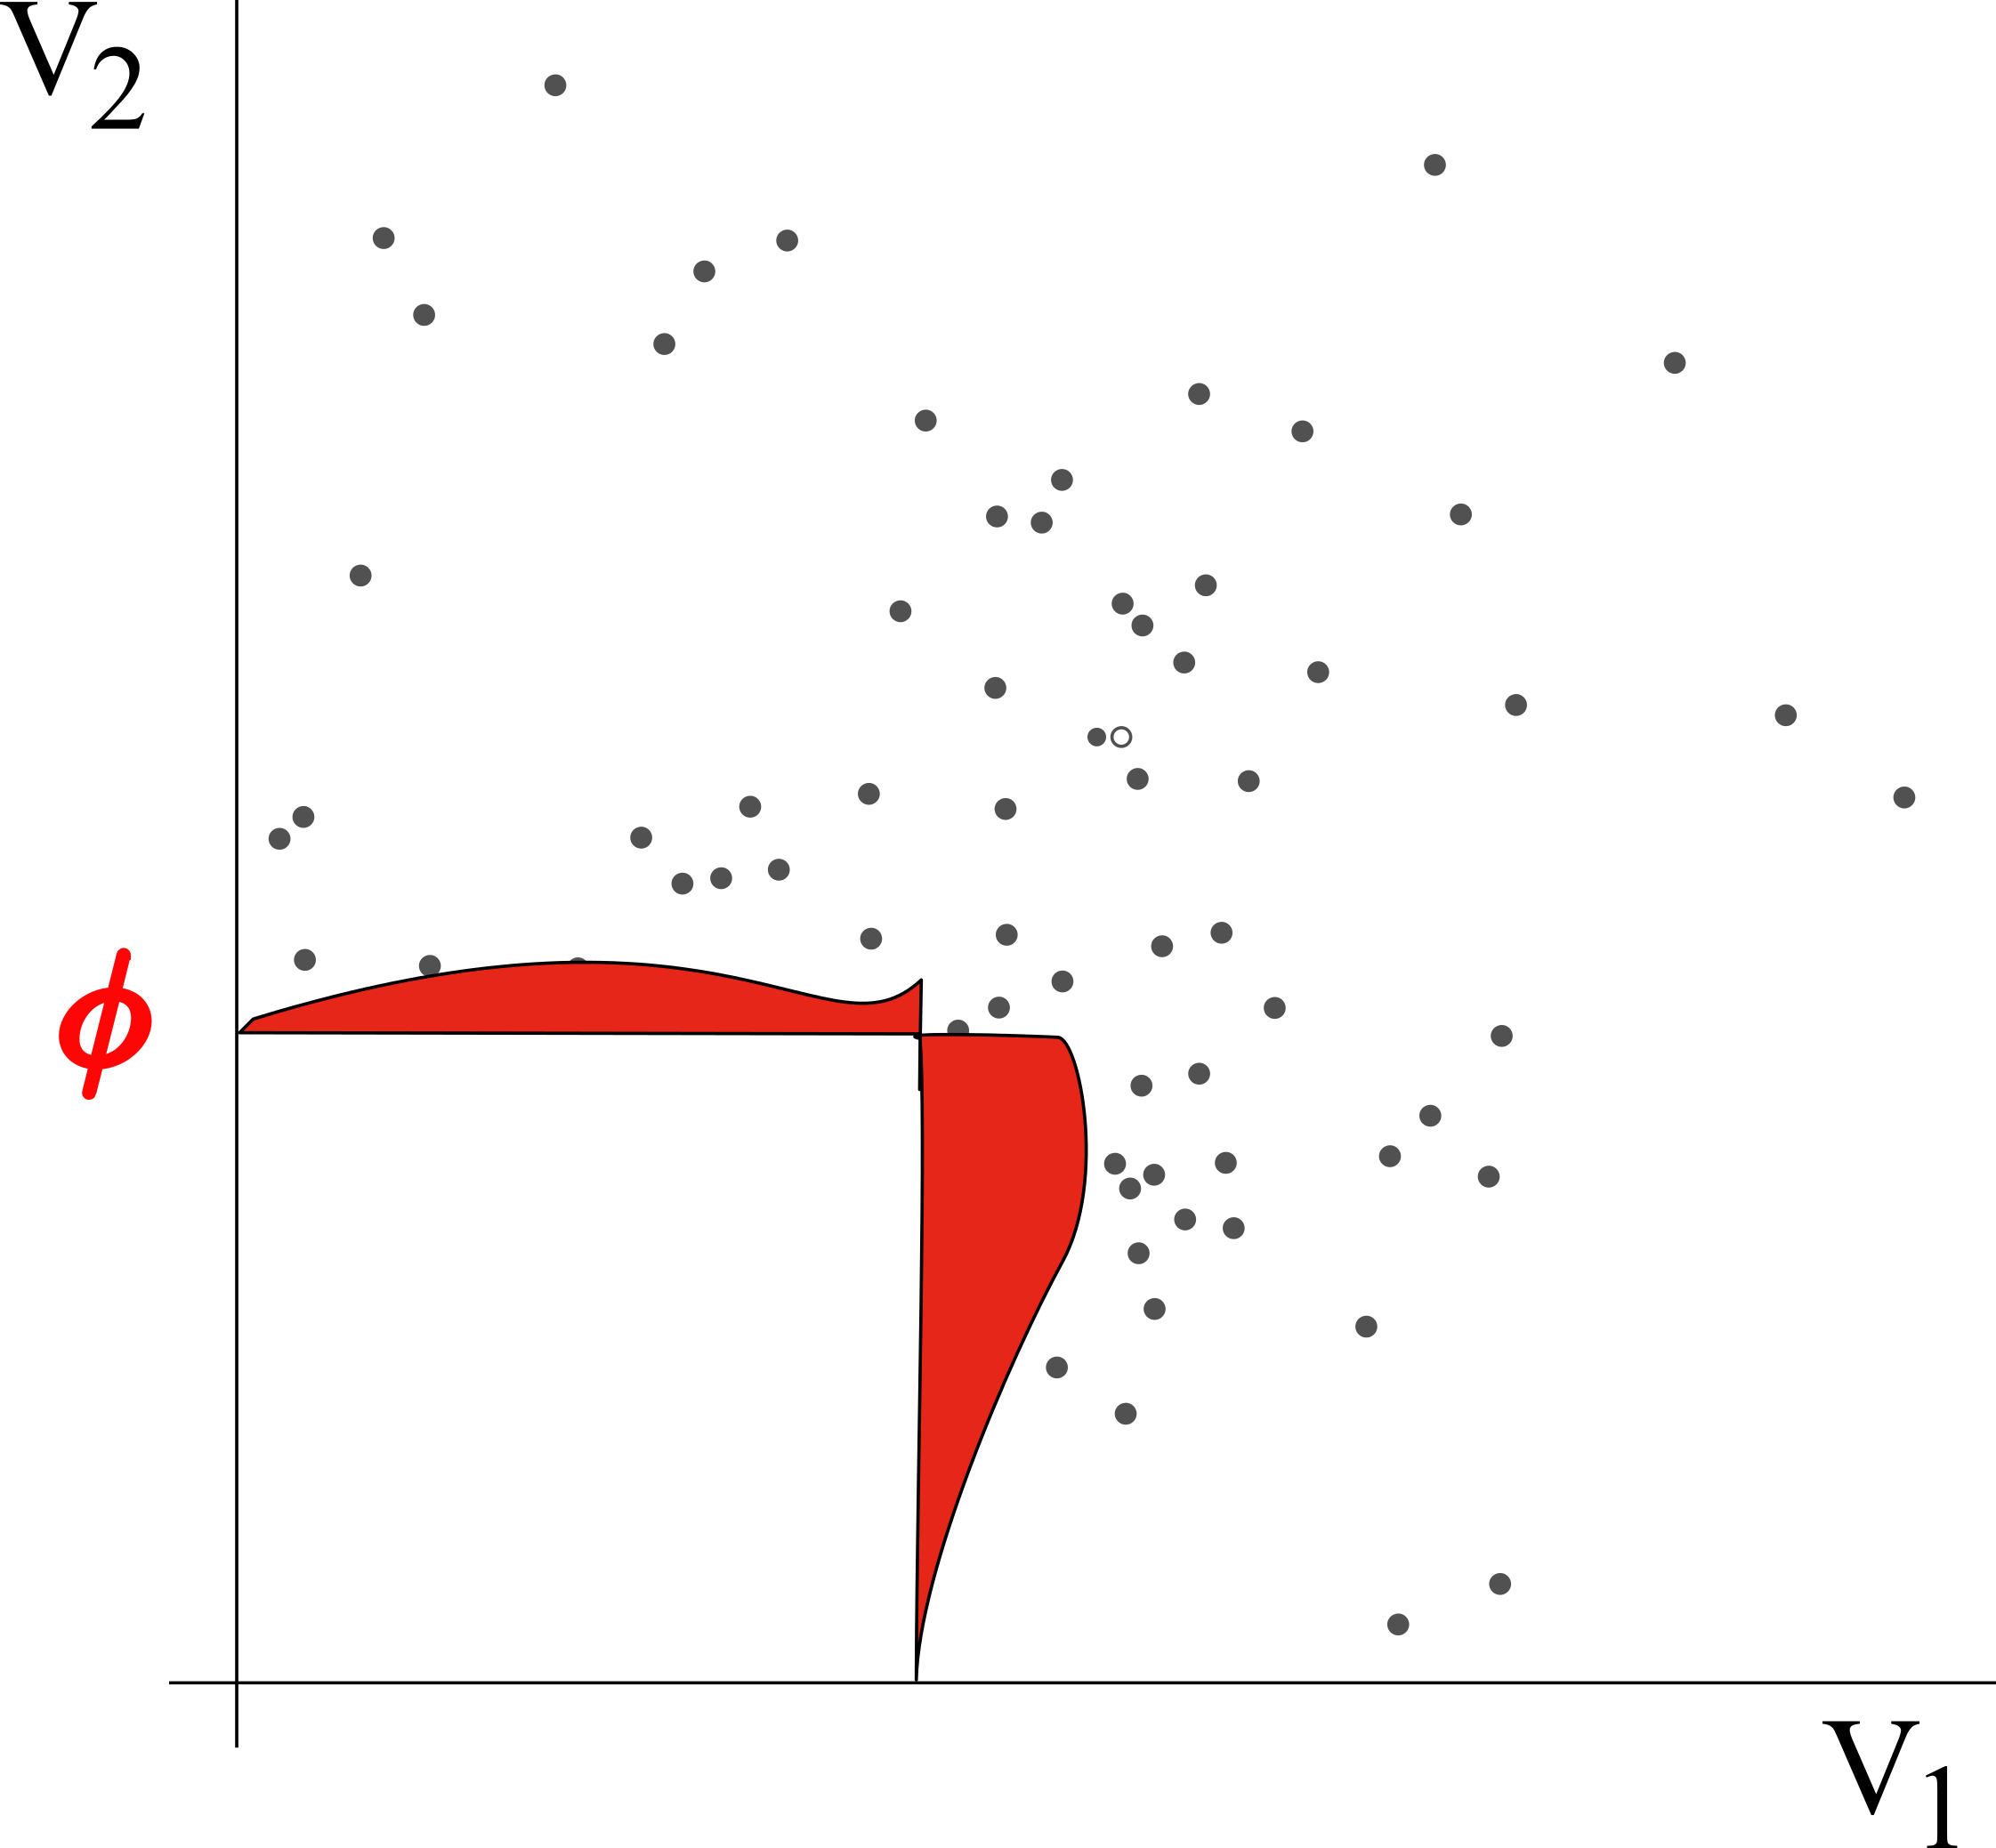
\includegraphics[scale=0.3]{sourcefigs/Example2D_depSquare.png}
      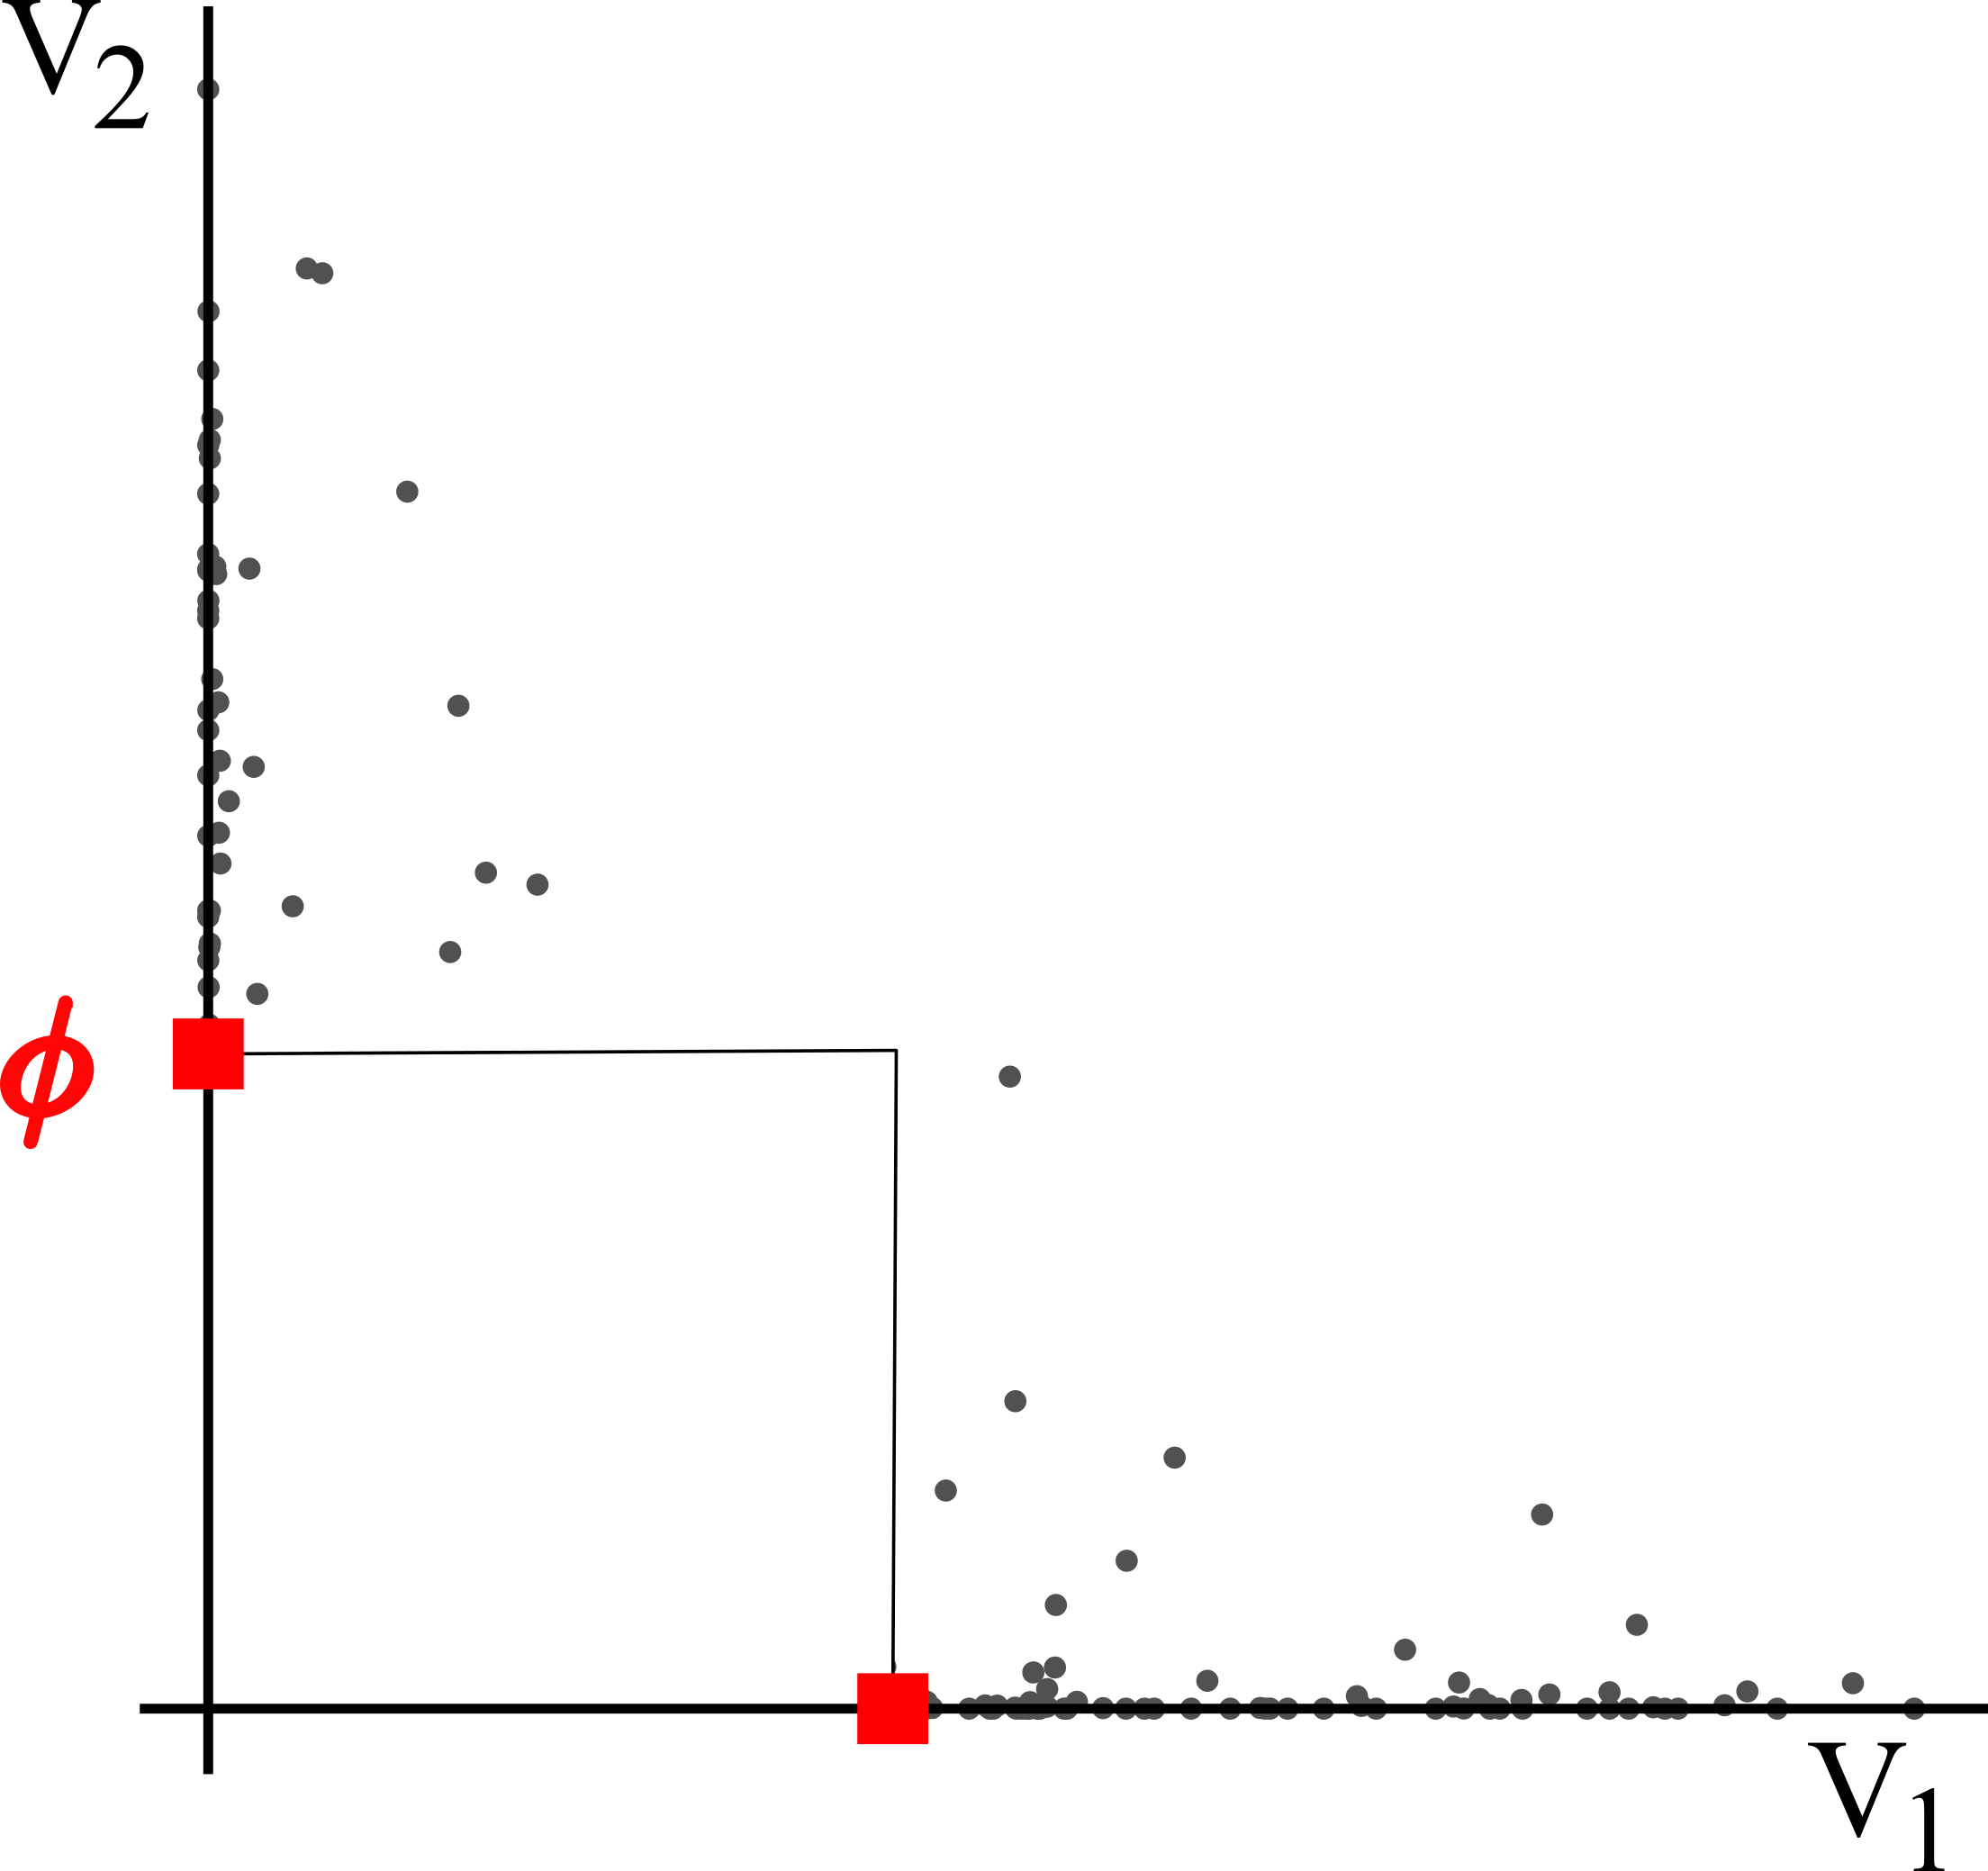
\includegraphics[scale=0.3]{sourcefigs/Example2D_indepSquare.png}
    \end{figure}
    \begin{itemize}
    \item Asymptotic dependence: $(V_1,V_2)$ may be large together.

\bigskip
vs
\bigskip

\item Asymptotic independence: only $V_1$ \emph{or} $V_2$ may be large.
    \end{itemize}
  \end{itemize}
\end{frame}


\begin{frame}
\frametitle{General Case}
  \begin{figure}
    \centering
    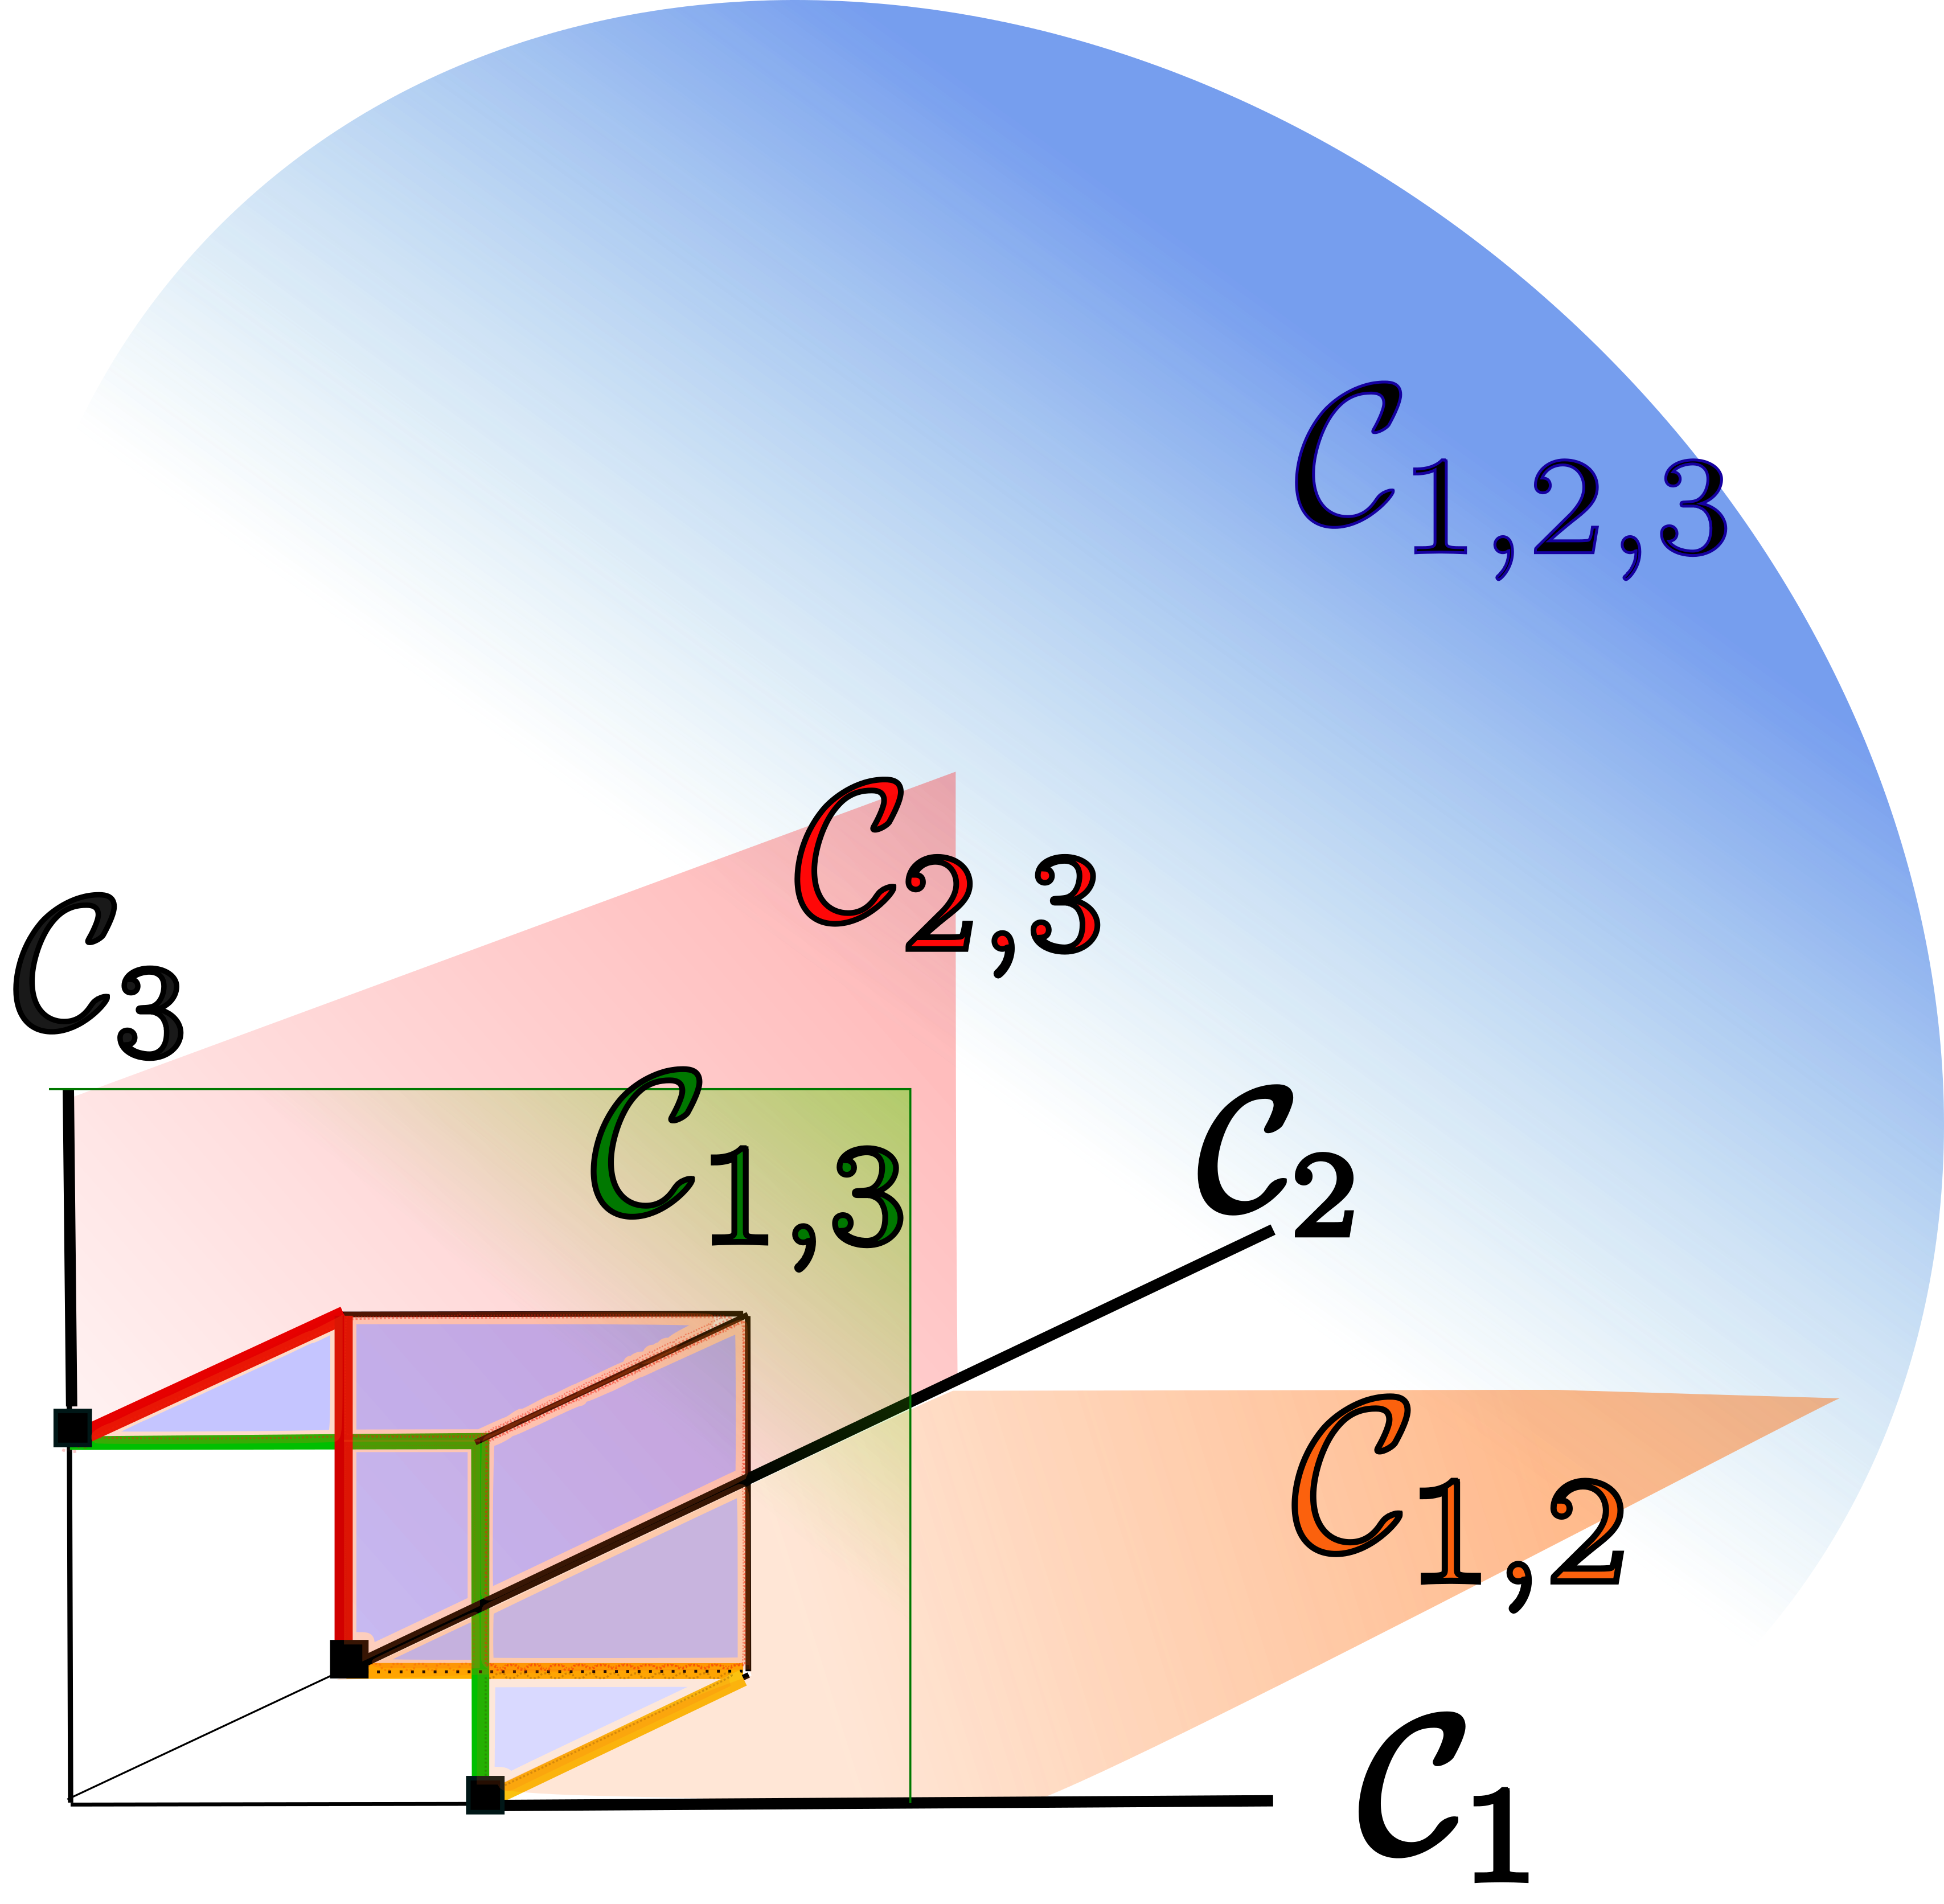
\includegraphics[width=0.4\linewidth]{sourcefigs/cone}
  \end{figure}
  \begin{itemize}
\item Sub-cones:  $\mathcal{C}_\alpha = \big\{\|v\|\ge 1,~~ v_i> 0 ~ (i\in\alpha),~~~  v_j = 0~(j\notin\alpha)\big\}$

\item   Corresponding sub-spheres: $\big\{\Omega_\alpha , \alpha\subset\{1,\dotsc,d\}\big\}$ ~~ ($\Omega_\alpha = \mathcal{C}_\alpha \cap \mathbf{S}_{d-1}$)
\end{itemize}
\end{frame}


% \begin{frame}
%   \frametitle{Joint extremes}
  
% \begin{figure}
% 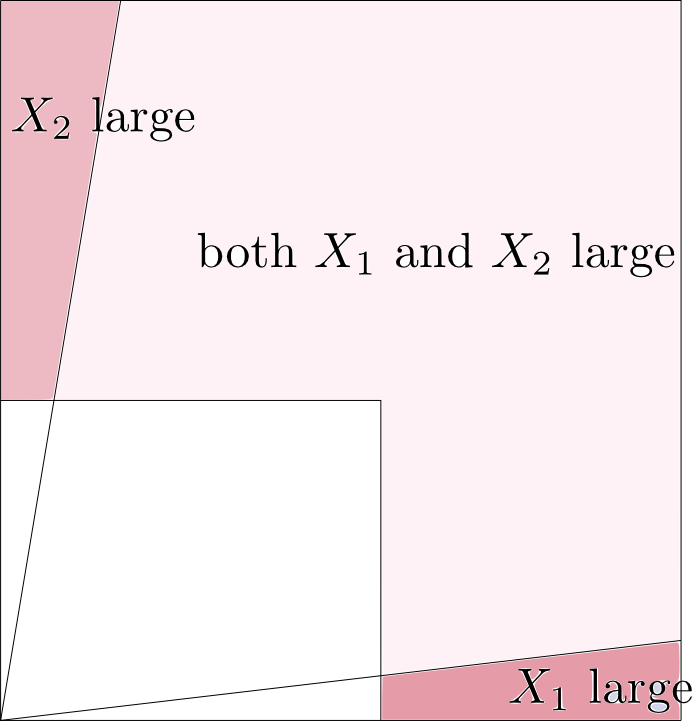
\includegraphics[width=0.68\linewidth]{sourcefigs/2DextremesIdea}
% \end{figure}
% \end{frame}


\begin{frame}
  \frametitle{Representation of extreme data}
\begin{itemize}
\item Natural decomposition of the angular measure :
$$
\Phi = \sum_{\alpha\subset\{1,\dotsc,d\}} \Phi_\alpha \text{~~~~~~~~~~~~~~~~~~with~~} \Phi_\alpha = \Phi_{|\Omega_\alpha} \leftrightarrow \mu_{|\mathcal{C}_\alpha}
$$


\item $\Rightarrow$ yields a representation
{\red
\begin{align*}
\mathcal{M} ~~&=~~ \Big\{~\Phi(\Omega_{\alpha}):~~~~ \emptyset \neq \alpha\subset\{1,\; \ldots,\; d \}~\Big\}  \\
&=~~ \Big\{~\mu(\mathcal{C}_{\alpha}):~~~~ \emptyset \neq \alpha\subset\{1,\; \ldots,\; d \}~\Big\}
\end{align*}
}  
% \begin{figure}
%     \centering
%     %\includegraphics[width=0.4\linewidth]{3D_anyH}\qquad 
%     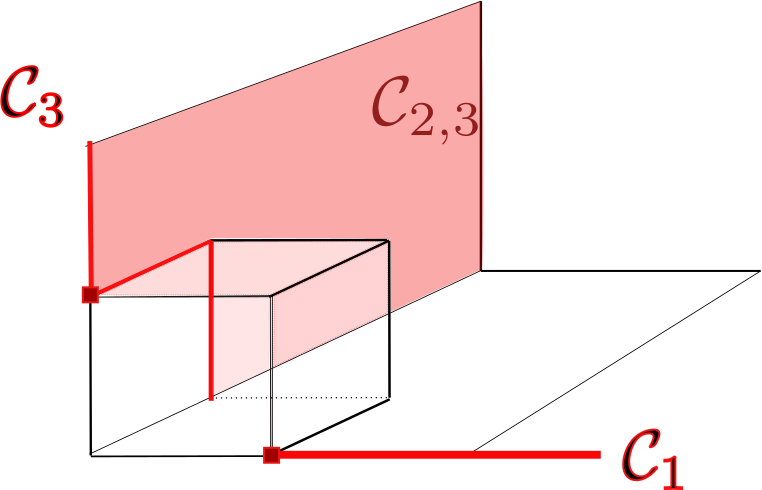
\includegraphics[width=0.3\linewidth]{sourcefigs/3D_sparseH}
%   \end{figure}

\item Assumption:  % $\Phi_\alpha = 0$ for $|\alpha|$ large,  and 
$\frac{\ud \mu_{|\mathcal{C}_\alpha}}{\ud v_\alpha} = O(1)$.\\~\\
 
\item Remark: Representation $\mathcal{M}$ is linear (after non-linear transform of the data $\mb X \to \mb V$).
\end{itemize}


\end{frame}

\begin{frame}
\frametitle{Sparse Representation ?}
  \begin{figure}
    \centering
    \includegraphics[width=0.4\linewidth]{sourcefigs/3D_anyH}\qquad 
    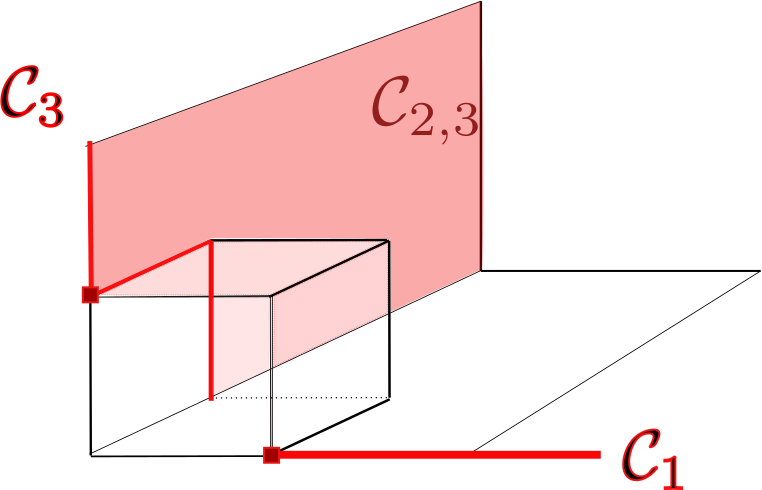
\includegraphics[width=0.4\linewidth]{sourcefigs/3D_sparseH} \\

 Full pattern : 
\hspace{3cm}   Sparse pattern  \\
{\footnotesize anything may happen}  \hspace{2cm} {\footnotesize ($V_1$ not large if
 $V_2$ or $V_3$ large)}
  \end{figure}
\end{frame}


\subsection{Estimation}

\begin{frame}
\frametitle{Problem: $\mathcal{M}$ is an \textbf{asymptotic} representation}

\begin{align*}
\mathcal{M} ~~=~~ \big\{~\Phi(\Omega_{\alpha}),~ \alpha~\big\} ~=~ \big\{~\mu(\mathcal{C}_{\alpha}),~ \alpha~\big\}
\end{align*}

is the restriction of an asymptotic measure 
\begin{align*}
\mu(A)=\lim_{t \to \infty} t \mathbb{P}[\mb V\in t~A]
\end{align*}
to a representative class of set $\{\mathcal{C}_\alpha,~\alpha\}$, but only the central sub-cone has positive Lebesgue measure!

\begin{minipage}{0.5\linewidth}
\centering
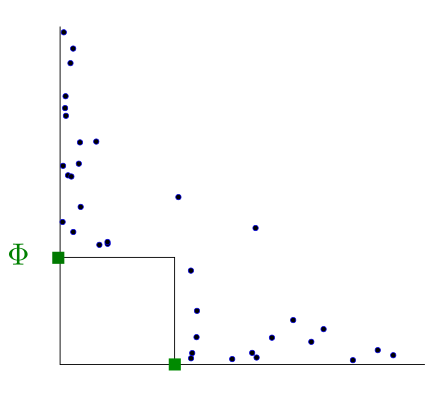
\includegraphics[scale=0.3]{sourcefigs/representation2D_problem}
\end{minipage}\hfill
\begin{minipage}{0.5\linewidth}
$\Rightarrow$ Cannot just do, for large $t$:
\begin{align*}
\Phi(\Omega_\alpha) = \mu(\mathcal{C}_\alpha) \simeq t \widehat{\mathbb{P}}(t \mathcal{C}_\alpha)
\end{align*}
\end{minipage}

\end{frame}

\begin{frame}
\frametitle{Solution}
 \textbf{Fix $\epsilon>0$. Affect data  $\epsilon$-close to an edge,
   to that edge. }

\begin{figure}[h]
  \centering
  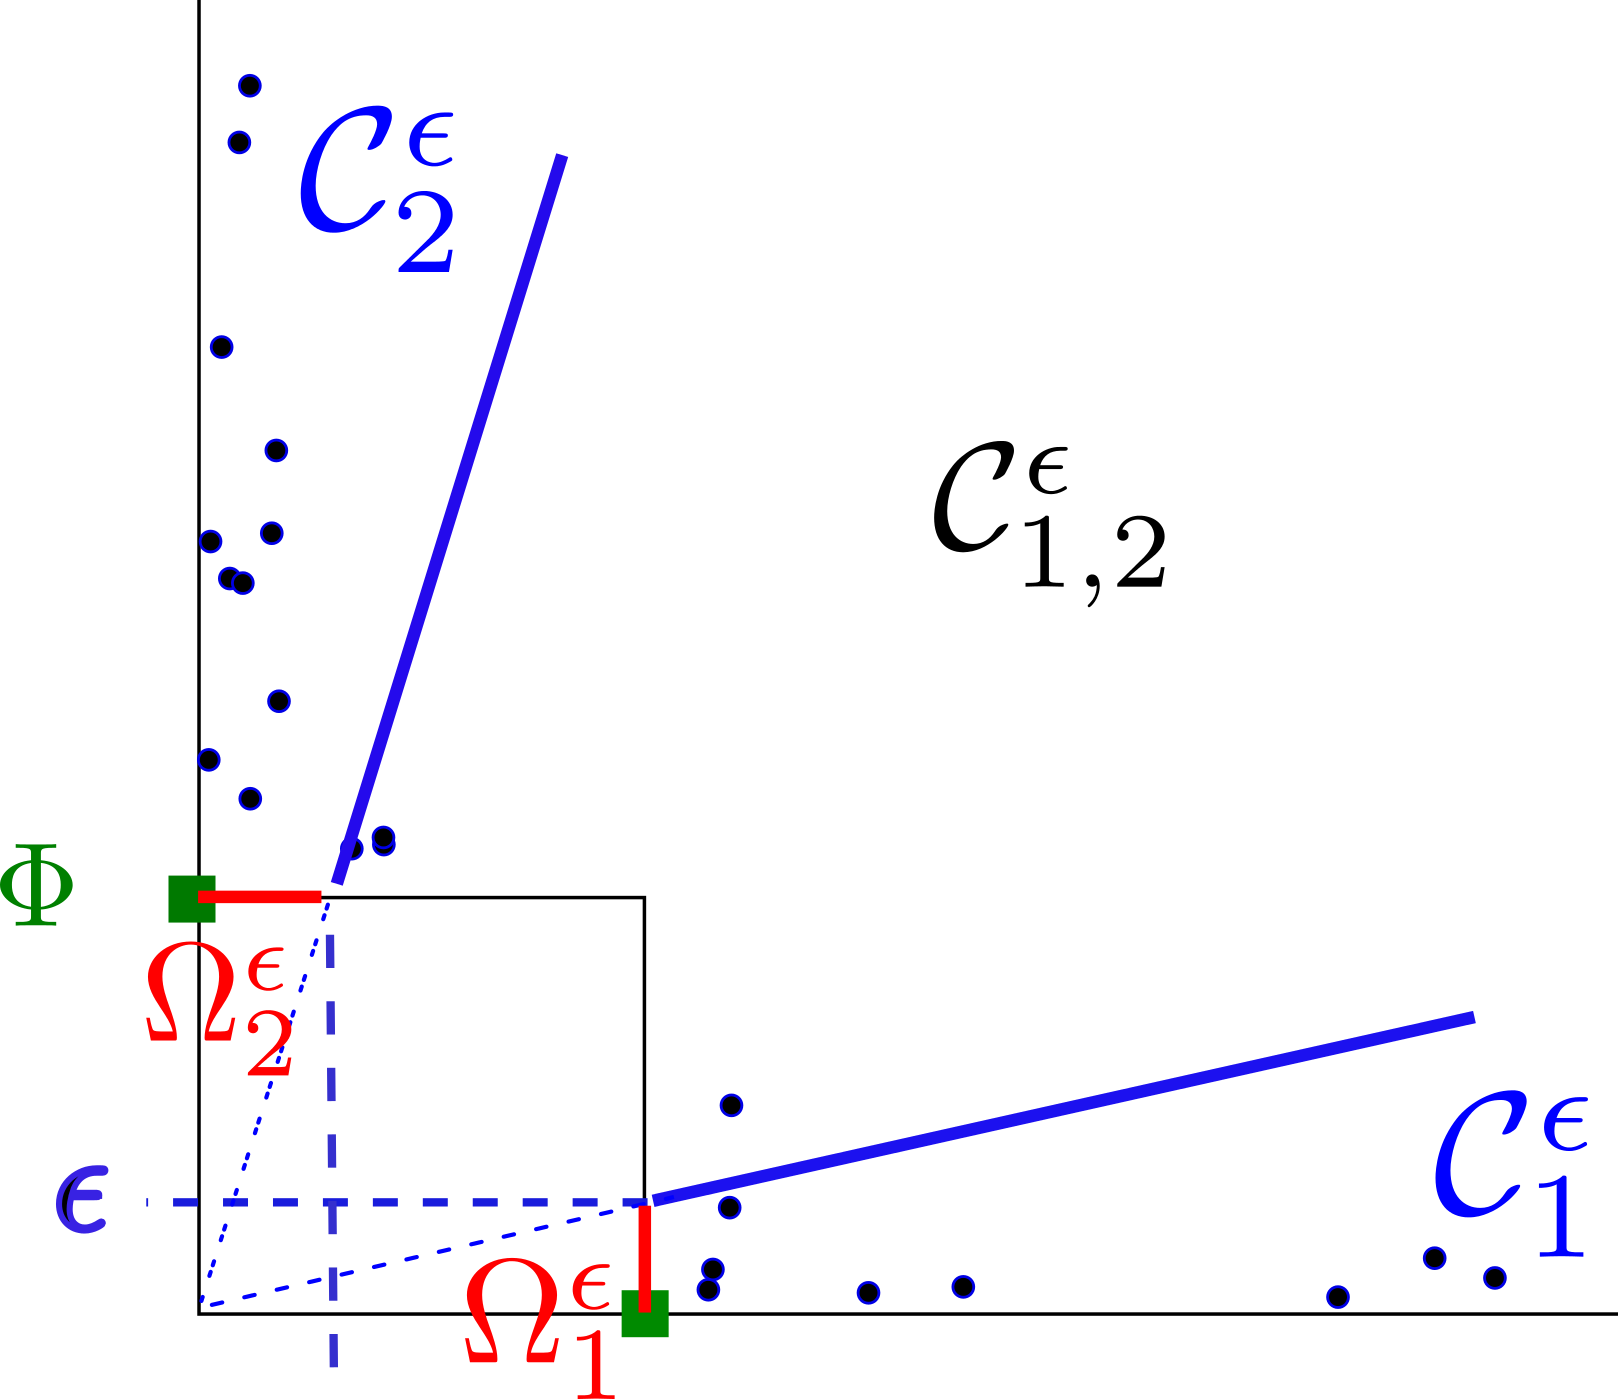
\includegraphics[scale=0.33]{sourcefigs/representation2D.png}
\end{figure}

\begin{align*}
\Omega_\alpha  \to  \Omega_\alpha^\epsilon &= \{v\in\mathbf{S}_{d-1}:
v_i>\epsilon\, (j\in\alpha),\,v_j \le \epsilon \,(j\notin\alpha) \}.  \\
\mathcal{C}_\alpha\to \mathcal{C}_\alpha^\epsilon&= \{t\,\Omega_\alpha^\epsilon,t\ge 1\}
\end{align*}
New partition of $\mathbf{S}_{d-1}$, compatible with non asymptotic data.
\end{frame}


\begin{frame}

$\hat V_i^j = \frac{1}{1- \hat F_j(X_{i}^j)}$ with 
$\hat F_j(X_{i}^j) =\frac{rank(X_i^j) -1}{n} $\\~\\

\begin{minipage}{0.5\linewidth}
\centering
$\Rightarrow$ get an natural estimate of $\Phi(\Omega_\alpha)$
\begin{align*}
&\widehat{\Phi}(\Omega_\alpha) := \frac{n}{k}\mathbb{P}_n( \hat V \in \frac{n}{k}\mathcal{C}_\alpha^\epsilon)\\
&(\frac{n}{k}~~ \text{large}, ~\epsilon~~ \text{small})
\end{align*}
\end{minipage}\hfill
\begin{minipage}{0.5\linewidth}
\centering
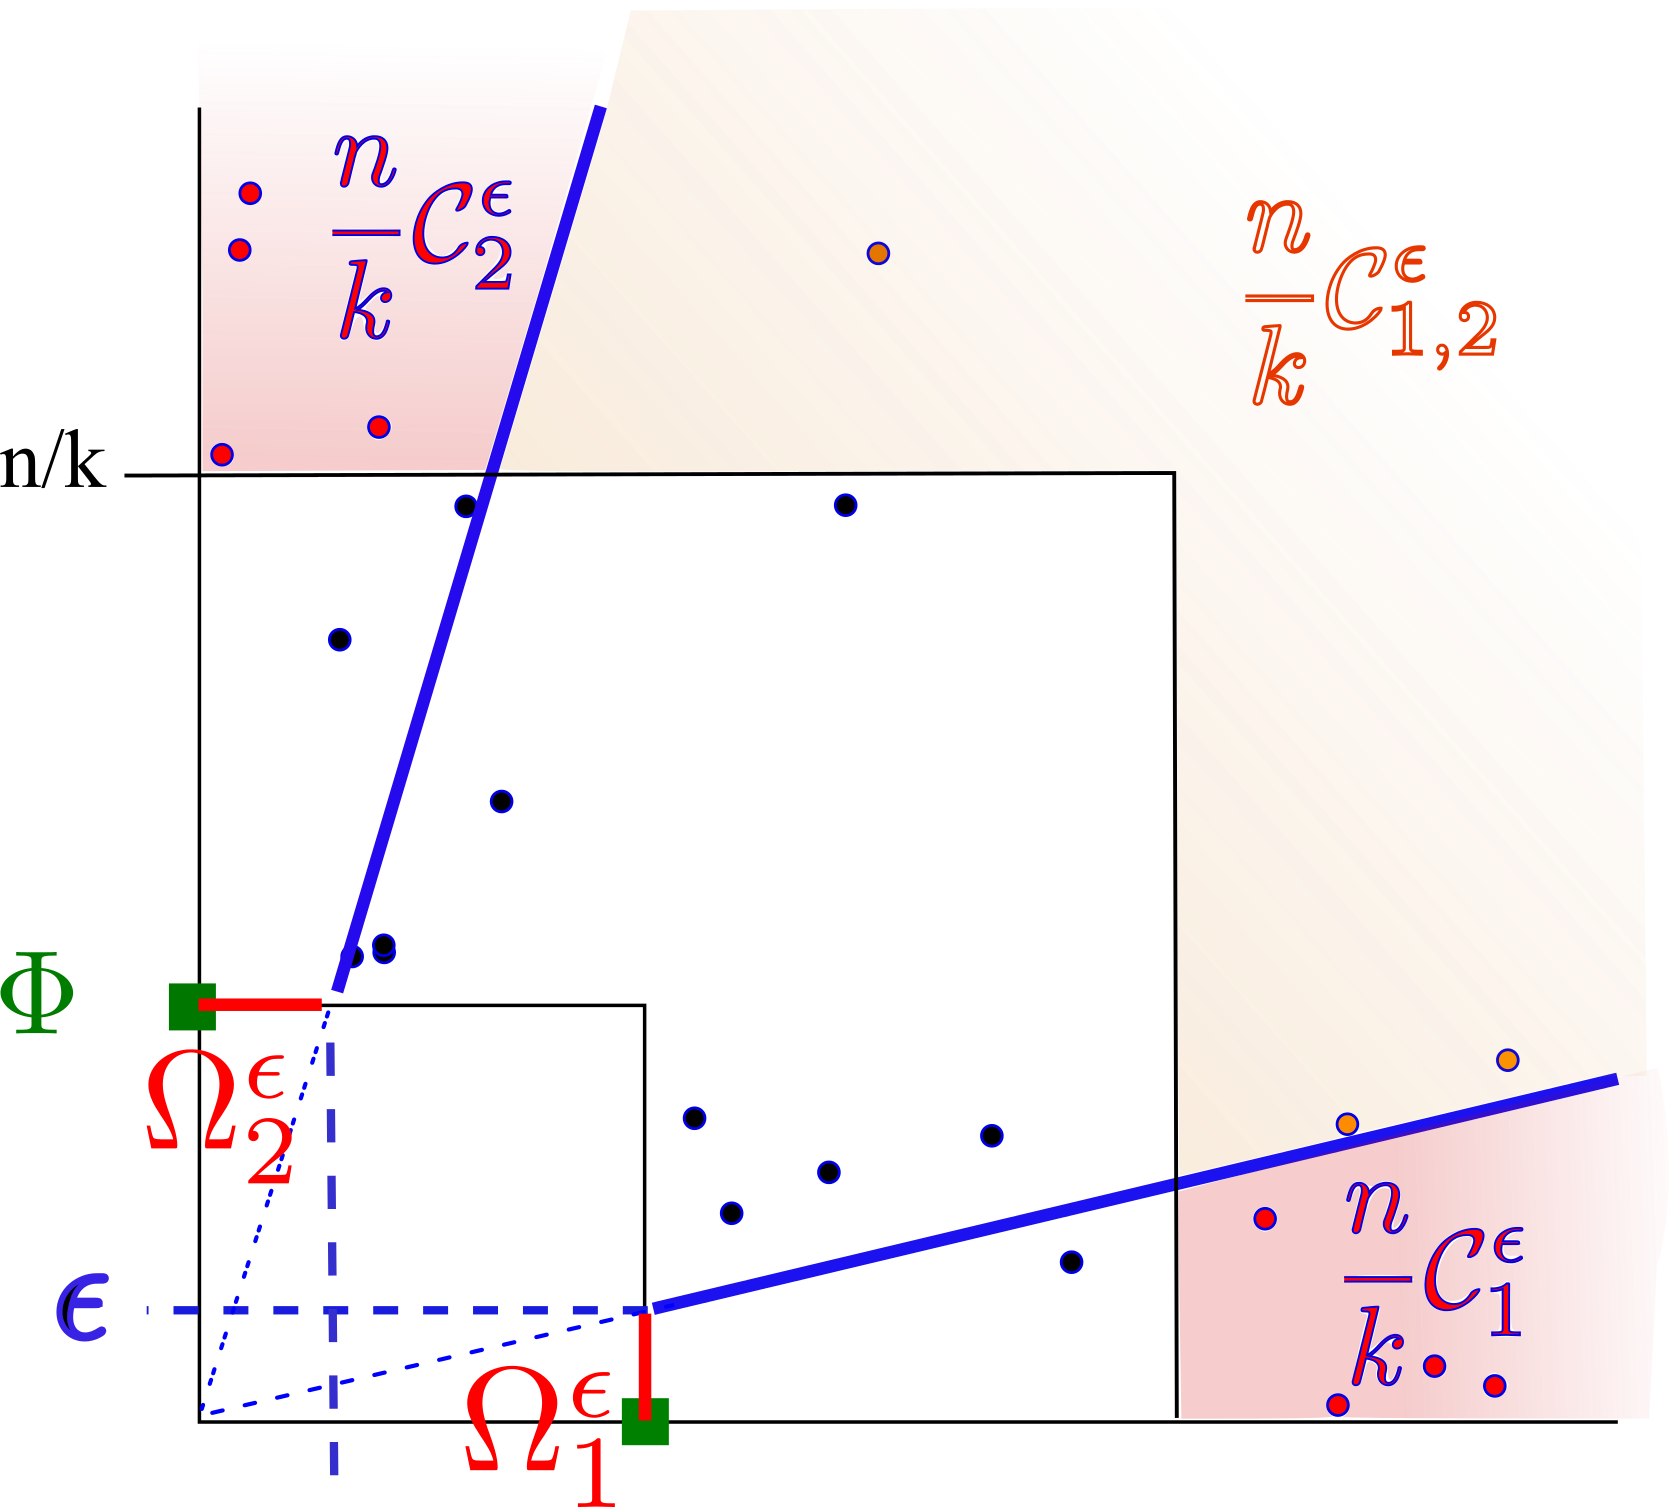
\includegraphics[scale=0.35]{sourcefigs/representation2D_nk.png}
\end{minipage}
~\\
$\Rightarrow$ we obtain
$$\widehat{\mathcal{M}}:=\big\{~\widehat{\Phi}(\Omega_{\alpha}),~ \alpha~\big\}$$
\end{frame}

\begin{frame}
\begin{theorem}
There is an absolute constant $C > 0$ such that for any $n>0,~ k>0,~ 0<\epsilon<1,~ \delta>0$ such that $0<\delta<e^{-k}$, with probability at least $1 - \delta$,
\begin{align*}
\|\widehat{\mathcal{M}}- \mathcal{M}\|_\infty
~\le~  C d \left( \sqrt{ \frac{1}{\epsilon k}\log\frac{d}{\delta}} + M d\epsilon \right) + \text{bias}(\epsilon, k, n),
\end{align*}
\end{theorem}

\textbf{Comments:}
% % \[
% % \begin{aligned}
% $
% \text{error}%\hat \Phi_n(\Omega_\alpha) - \Phi(\Omega_\alpha^0)|
% % |\mu_n(\mathcal{C}_\alpha^\epsilon) - \mu(\mathcal{C}_\alpha^0)|
% ~\le~  \Big( {\color{blue}\frac{C  d}{k^{1/4}} \sqrt{
%     \log\frac{d}{\delta}}} ~+~ %\
% {\color{violet}~ 5\sup_{0 \le x \le \frac{2 \sqrt k}{d}}\big|\frac{n}{k} \tilde F(\frac{k}{n}x)-\frac{n}{k} l ( \frac{k}{n} x)\big| }\Big)  
% $~\\~\\~\\
%
% $\Big(${\color{blue} variance $O(1/k^{1/4})$} + 
% {\color{violet} bias  }$\Big)$
\begin{itemize}


\item $C$: depends on $M=\sup$(density on subfaces)


\item  Existing litterature (for spectral measure) {\footnotesize \bf Einmahl
    Segers 09, Einmahl \emph{et.al.} 01}

  \begin{center}
$d=2$.    
  \end{center}
asymptotic behaviour, rates  in $1/\sqrt k$.\\
{\bf Here:} $1/\sqrt k\to  1/\sqrt{\epsilon k} + \epsilon$. Price to pay
for biasing our estimator with $\epsilon$.
\end{itemize} 
\end{frame}


\begin{frame}
\textbf{Theorem's proof}
\begin{enumerate}
\item \textbf{Maximal deviation on VC-class:}
\only<1>{ 
%Bound on the maximal deviation of $\mu_n$ on simple VC-class:
$$
\sup_{x\succeq {\epsilon}} |\mu_n - \mu| ([x,\infty[)  \le
{\color{blue} Cd\sqrt{\frac{2}{k}\log\frac{d}{\delta}} }  +
  {\color{violet} \text{bias}(\epsilon, k, n)% \text{bias}_{ \,\tilde F \leftrightarrow l, x\le 1/\epsilon}
  }
$$
\textbf{Tools}: Vapnik-Chervonenkis inequality adapted to small probability sets: bounds in ${\color{red}\sqrt{p}}\sqrt{\frac{1}{n}\log\frac{1}{\delta}}$\\~\\

On the VC class $\{ [\frac{n}{k} x, \infty]$, $x \ge \epsilon \}$

%   \begin{itemize}
%   \item 
%     \begin{itemize}
%     \item 
%    \item with nearly uniform
%     data $\hat U_{i,j} = 1 - \hat F_j(Y_{i,j}) ~( = 1/\hat X_{i,j})$.
%     \end{itemize}
% % $\exists C, \text{ indep from } n, d$, s.t., with proba $1-\delta$,
% \end{itemize}
}
\only<2>{\item \textbf{Decompose error:}
  \[|\mu_n(\mathcal{C}_\alpha^\epsilon) - \mu(\mathcal{C}_\alpha)| \le 
\underbrace{|\mu_n- \mu|(\mathcal{C}_\alpha^\epsilon)}_A +
\underbrace{ |\mu(\mathcal{C}_{\alpha}^\epsilon) - \mu(\mathcal{C}_\alpha) |}_B \]\\
\begin{itemize}
% \item 
 % Restriction to cube $[0,L]$, 
\item $A : $ First step.
\item % $B  = O( M d^2 (\epsilon )^{d-\alpha}) $ $\to $ OK with boundedness
  % assumption.
  $B  : $ density on $\mathcal{C}_\alpha^\epsilon \times Lebesgue$ : small \\~\\%% O( M (d^2 \epsilon + (1+\epsilon)^d -1)) $ % $\to $ OK with boundedness
   % assumption.

% %% $A=O\Big(~ 2^\alpha  E  + M \alpha d (\epsilon L)  + Md^2
%                                  (1+ \epsilon L )^{d}-1   
% +
%   \frac{1}{L}~\Big)$ \\

%\item Optimize in $L, \epsilon \Rightarrow \epsilon=d/\sqrt k$  \\
%explains the $k^{1/4}$ loss compared with low dimension.

\end{itemize}
}
\end{enumerate}
\end{frame}


\begin{frame}
\begin{center}

% \begin{minipage}{0.95\linewidth}

\begin{algorithmic} 
DAMEX in $O(dn\log n)$

\STATE {\bf Input:} parameters $\epsilon>0$,~~ $k = k(n)$,~~ %$\Phi_{\min}\geq 0$.
\STATE Standardize \emph{via} marginal rank-transformation: $\hat V_i := \big (1/(1- \hat F_j (X_i^j))\big)_{j=1,\ldots,d}$~. 
\STATE Assign to each $\hat V_i$ the cone $\frac{n}{k}\mathcal{C}_\alpha^\epsilon$
  it belongs to.  
\STATE $\Phi_n^{\alpha,\epsilon} := \widehat{\Phi}(\Omega_\alpha) = \frac{n}{k}\mathbb{P}_n( \hat V \in \frac{n}{k}\mathcal{C}_\alpha^\epsilon)$
the estimate of the $\alpha$-mass of $\Phi$.
   
\STATE {\bf Output:} (sparse) representation of the dependence
  structure %$(\mu_n^{\alpha,\epsilon})_{\alpha\subset\{1,\ldots, d\}, \mu_n^{\alpha,\epsilon}>\mu_{\min}}$.

\begin{align*}
\widehat{\mathcal{M}} := (\Phi_n^{\alpha,\epsilon})_{\alpha\subset\{1,\ldots, d\}, \Phi_n^{\alpha,\epsilon}>\Phi_{\min}}
\end{align*}

\end{algorithmic}
% \end{minipage}

\end{center}
\end{frame}


\begin{frame}
\frametitle{Application to Anomaly Detection}

After standardization of marginals: 
$\mathbb{P}[R> r  ,\mb W \in B ]  \simeq \frac{1}{r}\,\Phi(B)$ \\~\\
 $\rightarrow$ scoring function = $\Phi_n^\epsilon$  $\times 1/r:$
$$s_n(\mb x):= (1/\|\hat T(\mb x)\|_\infty) \sum_{\alpha }\Phi_n^{\alpha, \epsilon} \mathds{1}_{\hat T(\mb x) \in \mathcal{C}_\alpha^\epsilon}.$$~\\
 where $T: \mb X \mapsto \mb V$ ~~~~~~~~~($V_{j} = \frac{1}{1- F_j (X_{j})} $)

  \begin{figure}
    \centering
    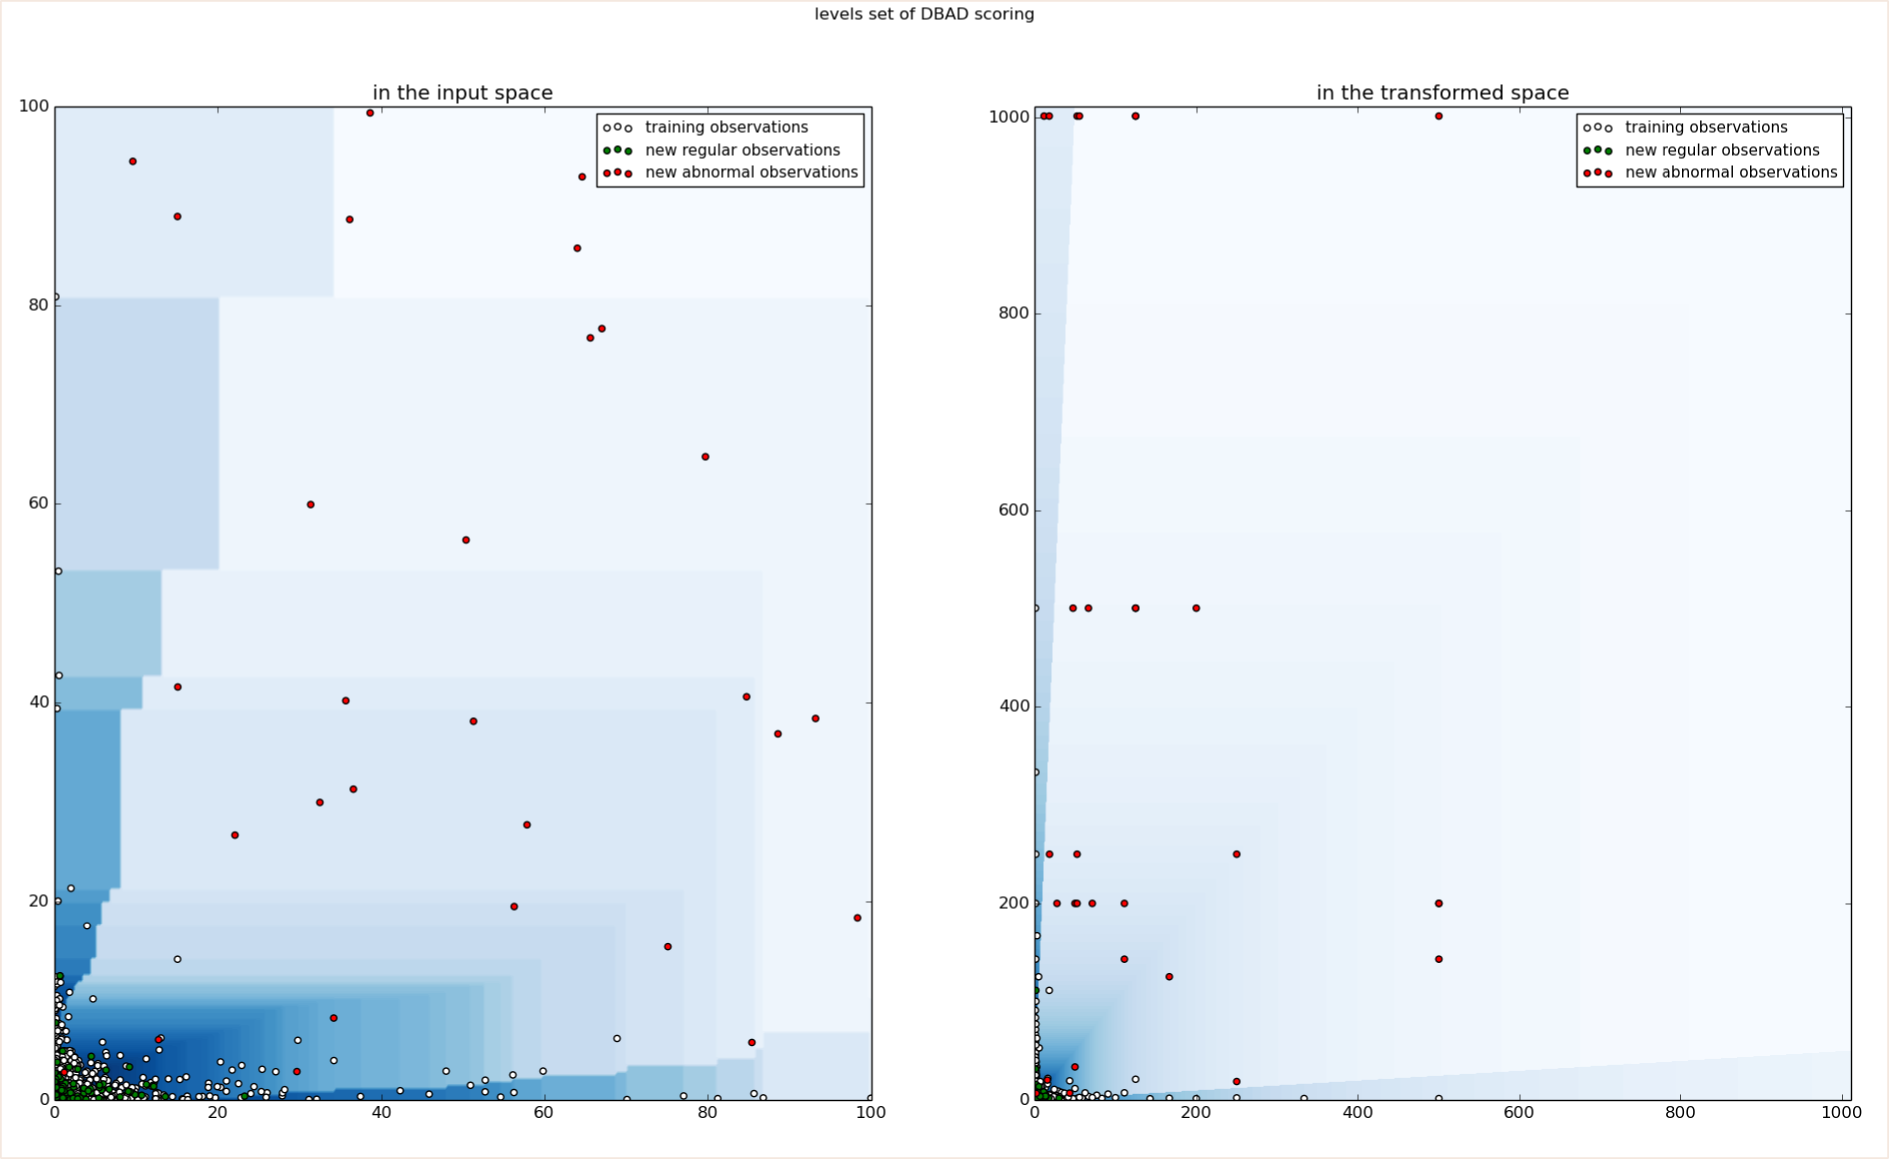
\includegraphics[scale=0.15, trim=2cm 0cm 2cm 1cm]{sourcefigs/DBAD}
  \end{figure}

\end{frame}


\subsection{Experiments}


\begin{frame}
\begin{table}[h]
\centering
\begin{tabular}{|l|cc|}
  \hline
  ~           & number of samples  & number of features \\
  shuttle     & 85849              & 9                  \\
  forestcover & 286048             & 54                 \\
  SA          & 976158             & 41                 \\
  SF          & 699691             & 4                  \\
  http        & 619052             & 3                  \\
  smtp        & 95373              & 3                  \\
  \hline
\end{tabular}
\caption{Datasets characteristics}
\label{table:data}
\end{table}
\end{frame}


% \begin{frame}
% \begin{figure}[H]
%   \centering
%   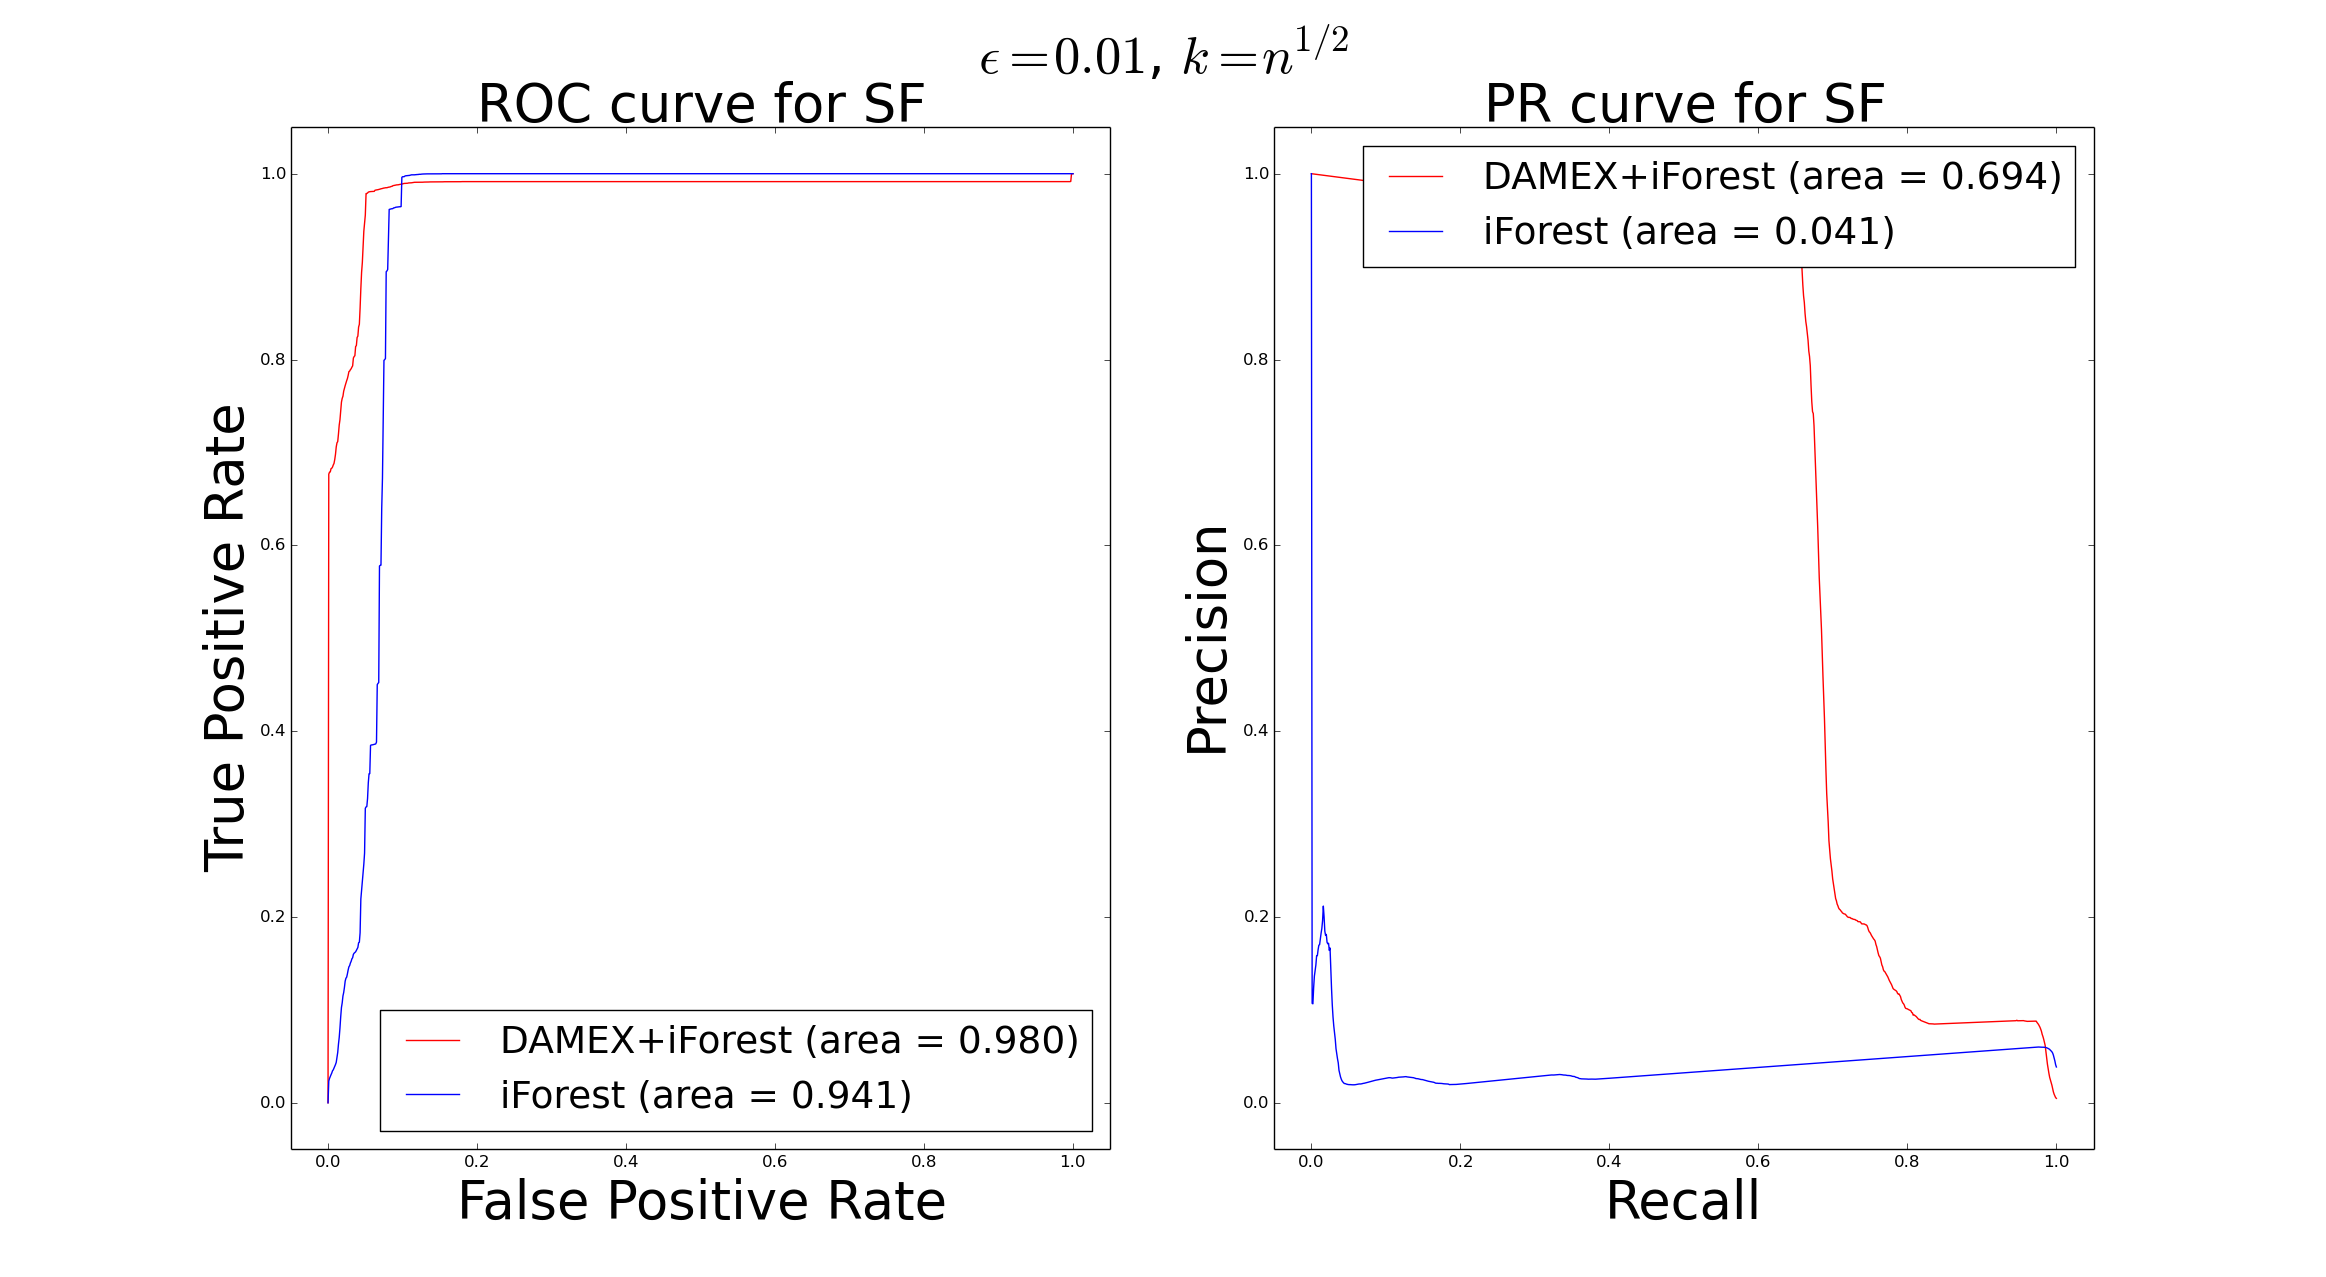
\includegraphics[width = 1. \textwidth]{sourcefigs/SF-4d-lb-semi-supervised-average}
%   \caption{ROC and PR curve on SF dataset}
%   \label{SF}
% \end{figure}
% \end{frame}



% \begin{frame}
% \begin{figure}[H]
%   \centering
%   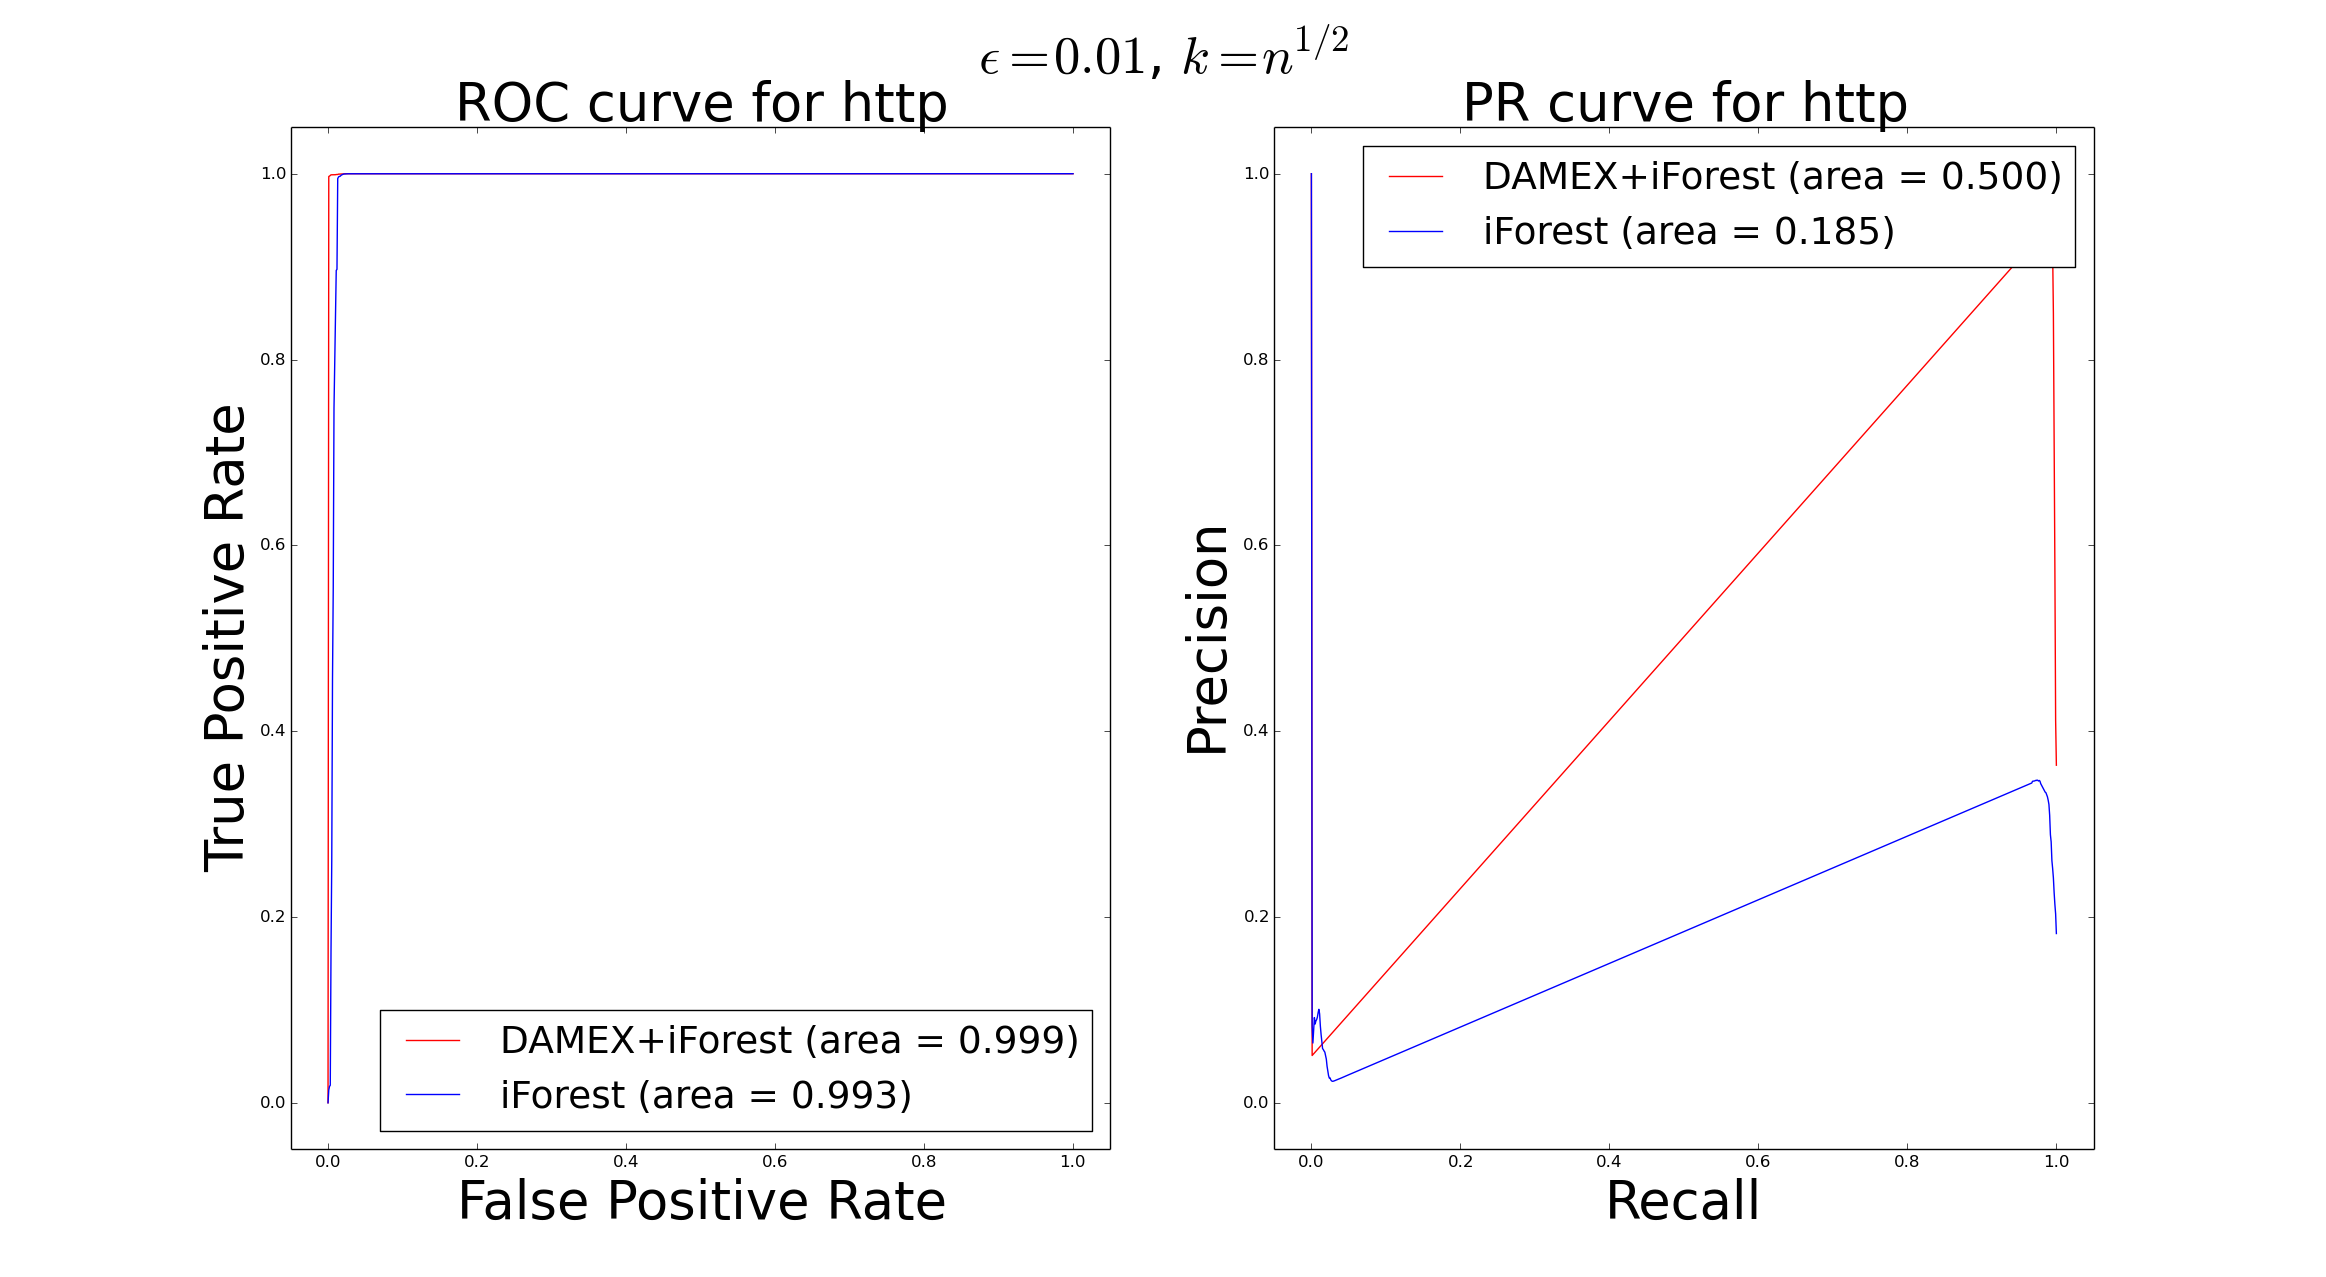
\includegraphics[width = 1. \textwidth]{sourcefigs/http-3d-semi-supervised-average}
%   \caption{ROC and PR curve on http dataset}
%   \label{http}
% \end{figure}
% \end{frame}


% \begin{frame}
% \begin{figure}[H]
%   \centering
%   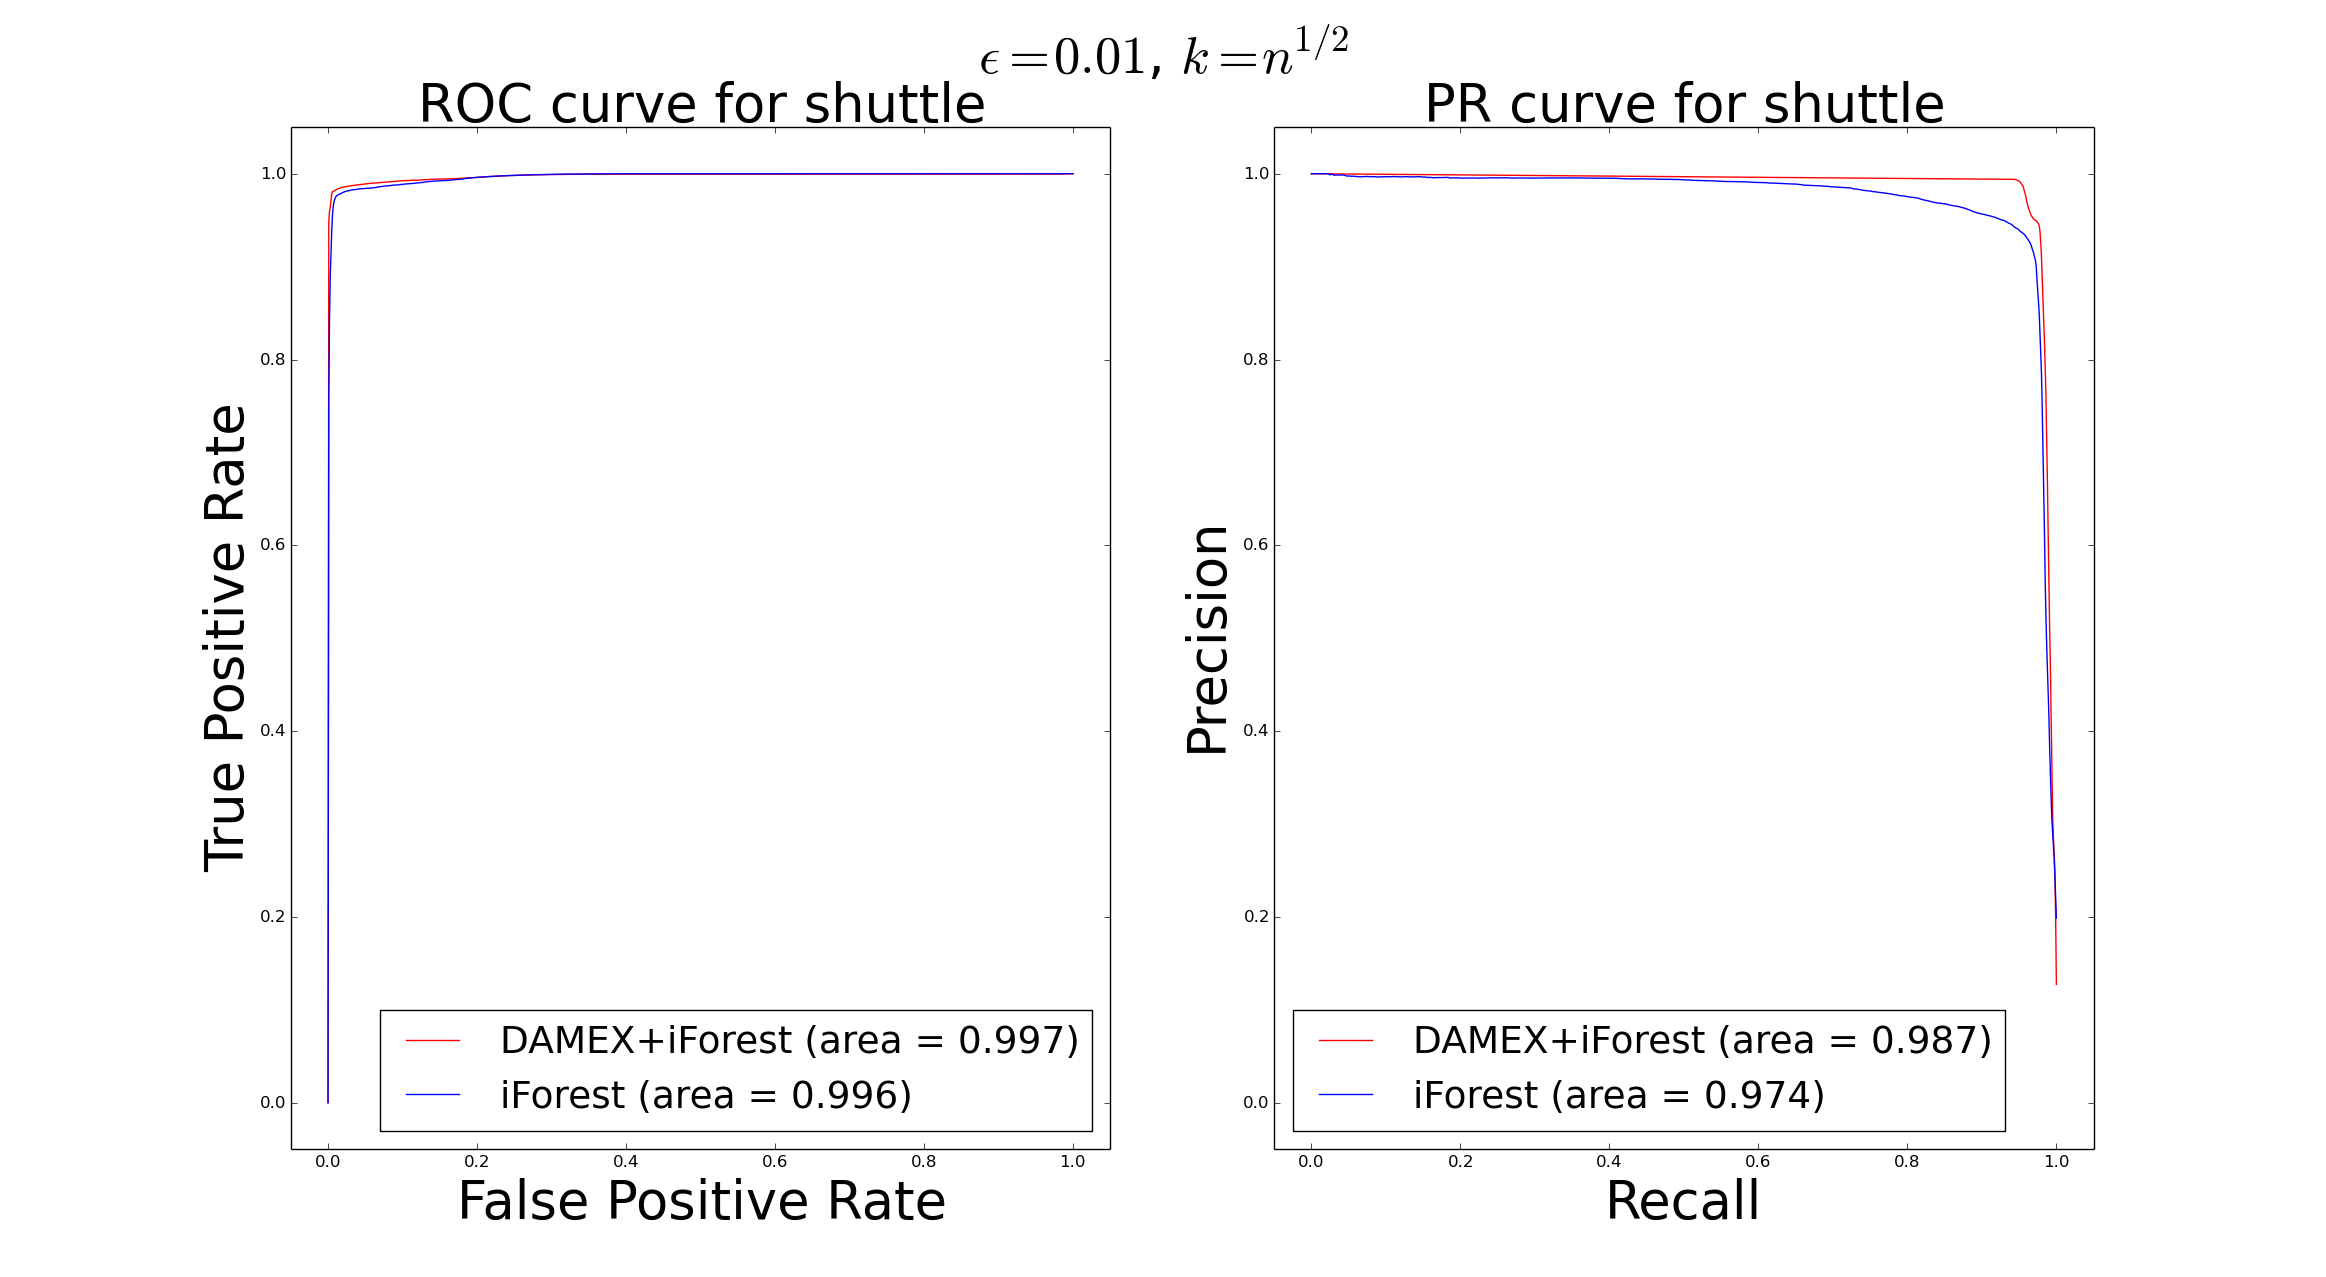
\includegraphics[width = 1. \textwidth]{sourcefigs/shuttle-semi-supervised-average}
%   \caption{ROC and PR curve on shuttle dataset}
%   \label{shuttle}
% \end{figure}
% \end{frame}

% \begin{frame}
% \begin{figure}[H]
%   \centering
%   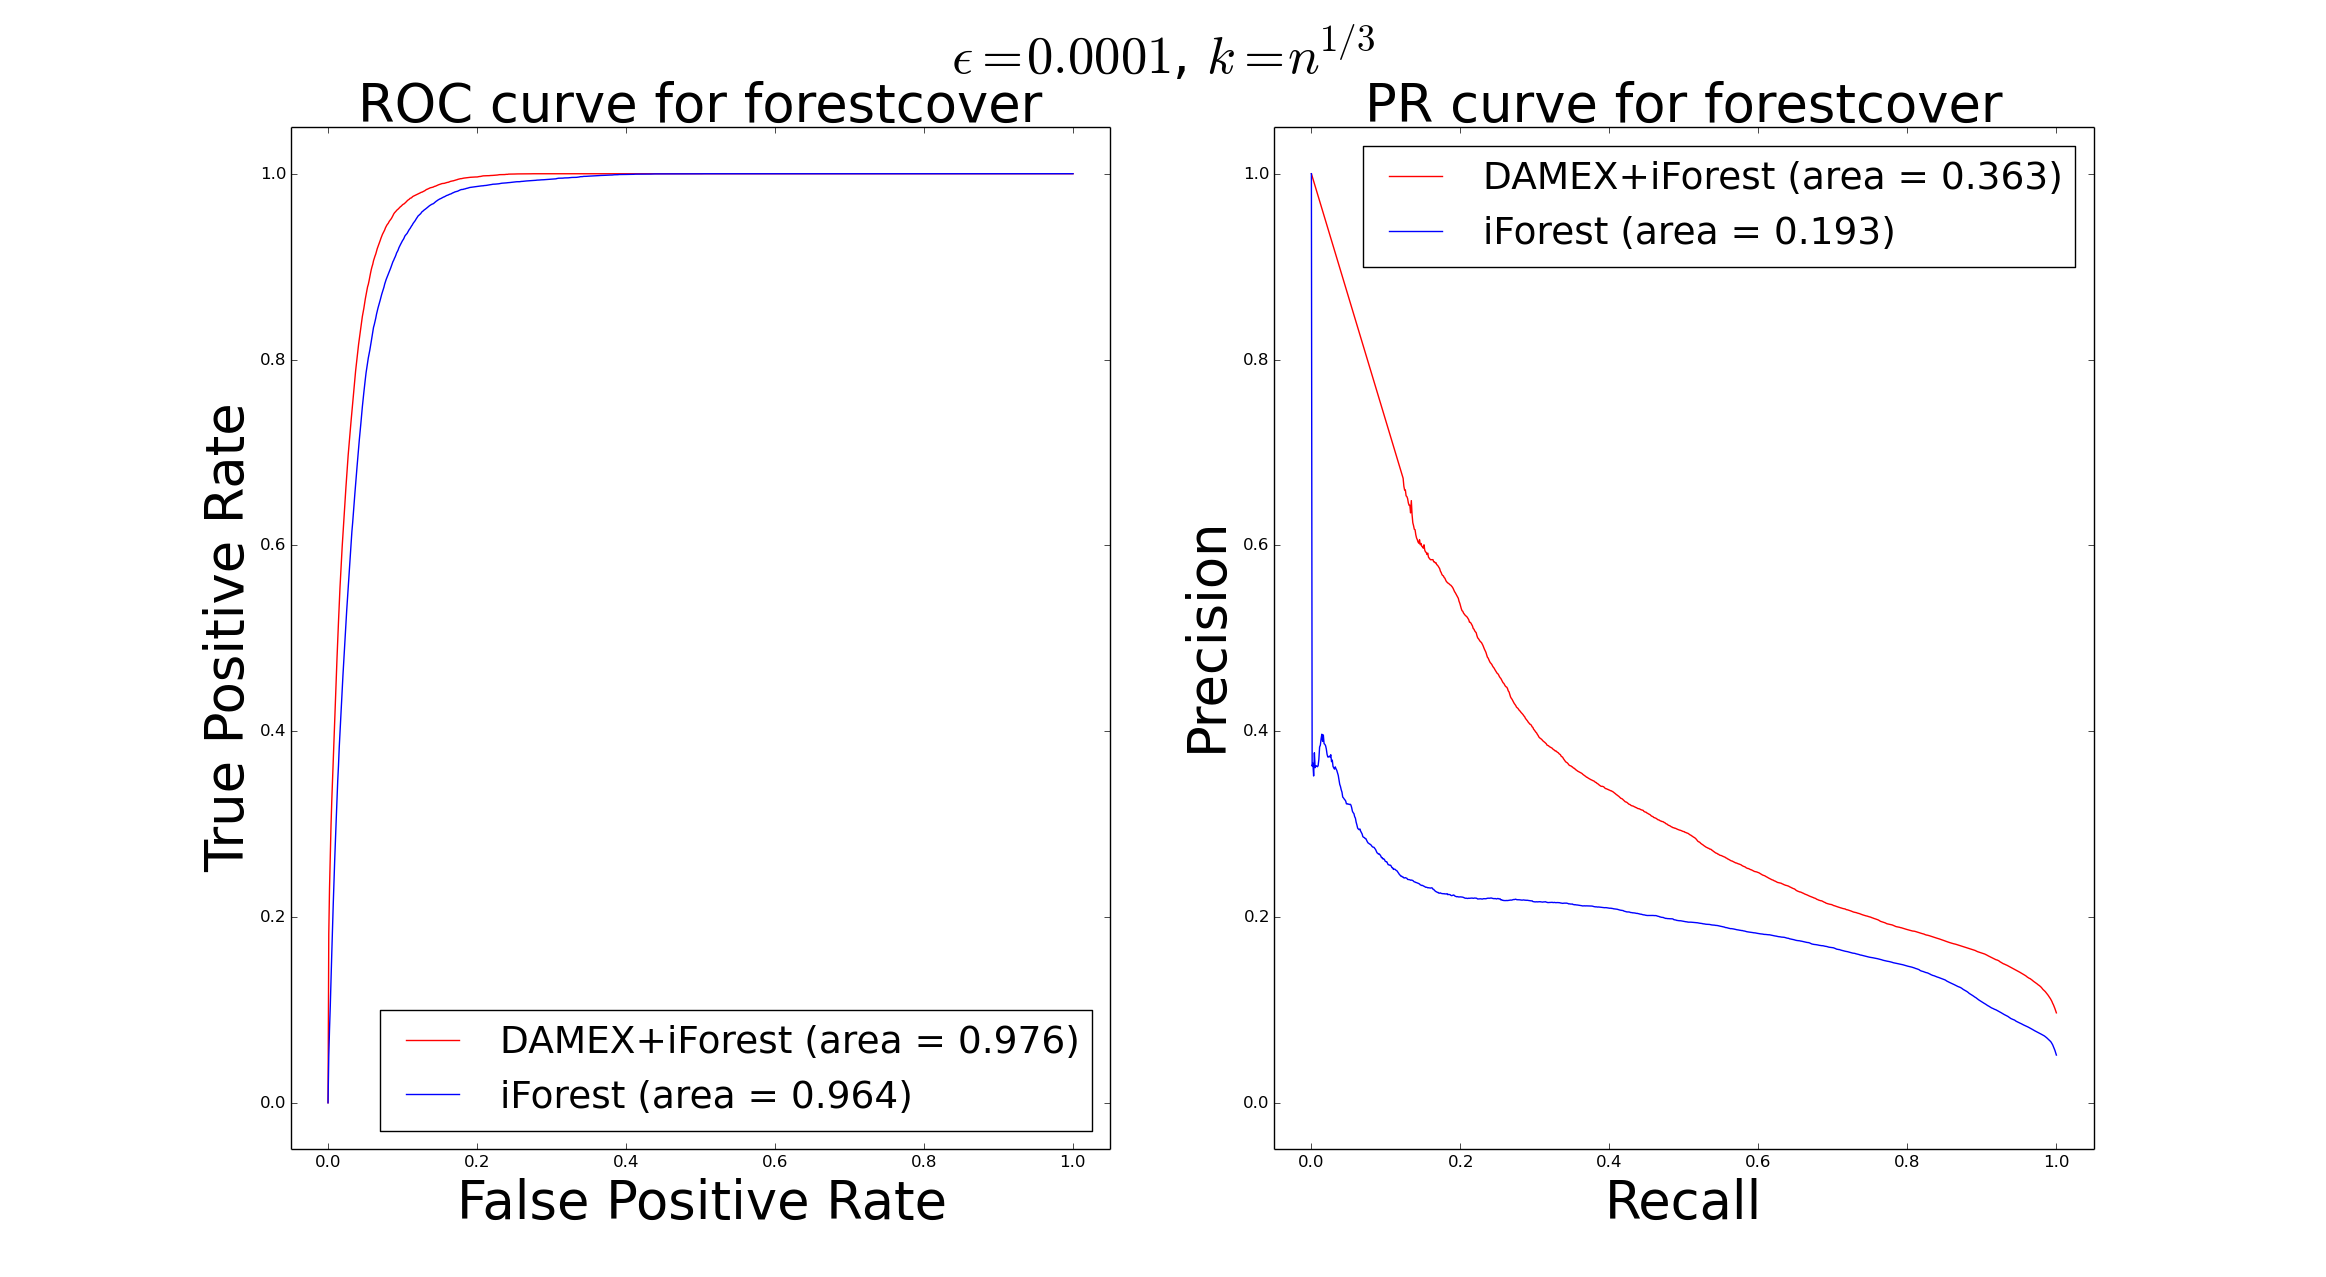
\includegraphics[width = 1. \textwidth]{sourcefigs/forestcover-semi-supervised-average}
%   \caption{ROC and PR curve on forestcover dataset}
%   \label{forestcover}
% \end{figure}
% \end{frame}


% \begin{frame}
% \begin{figure}[H]
%   \centering
%   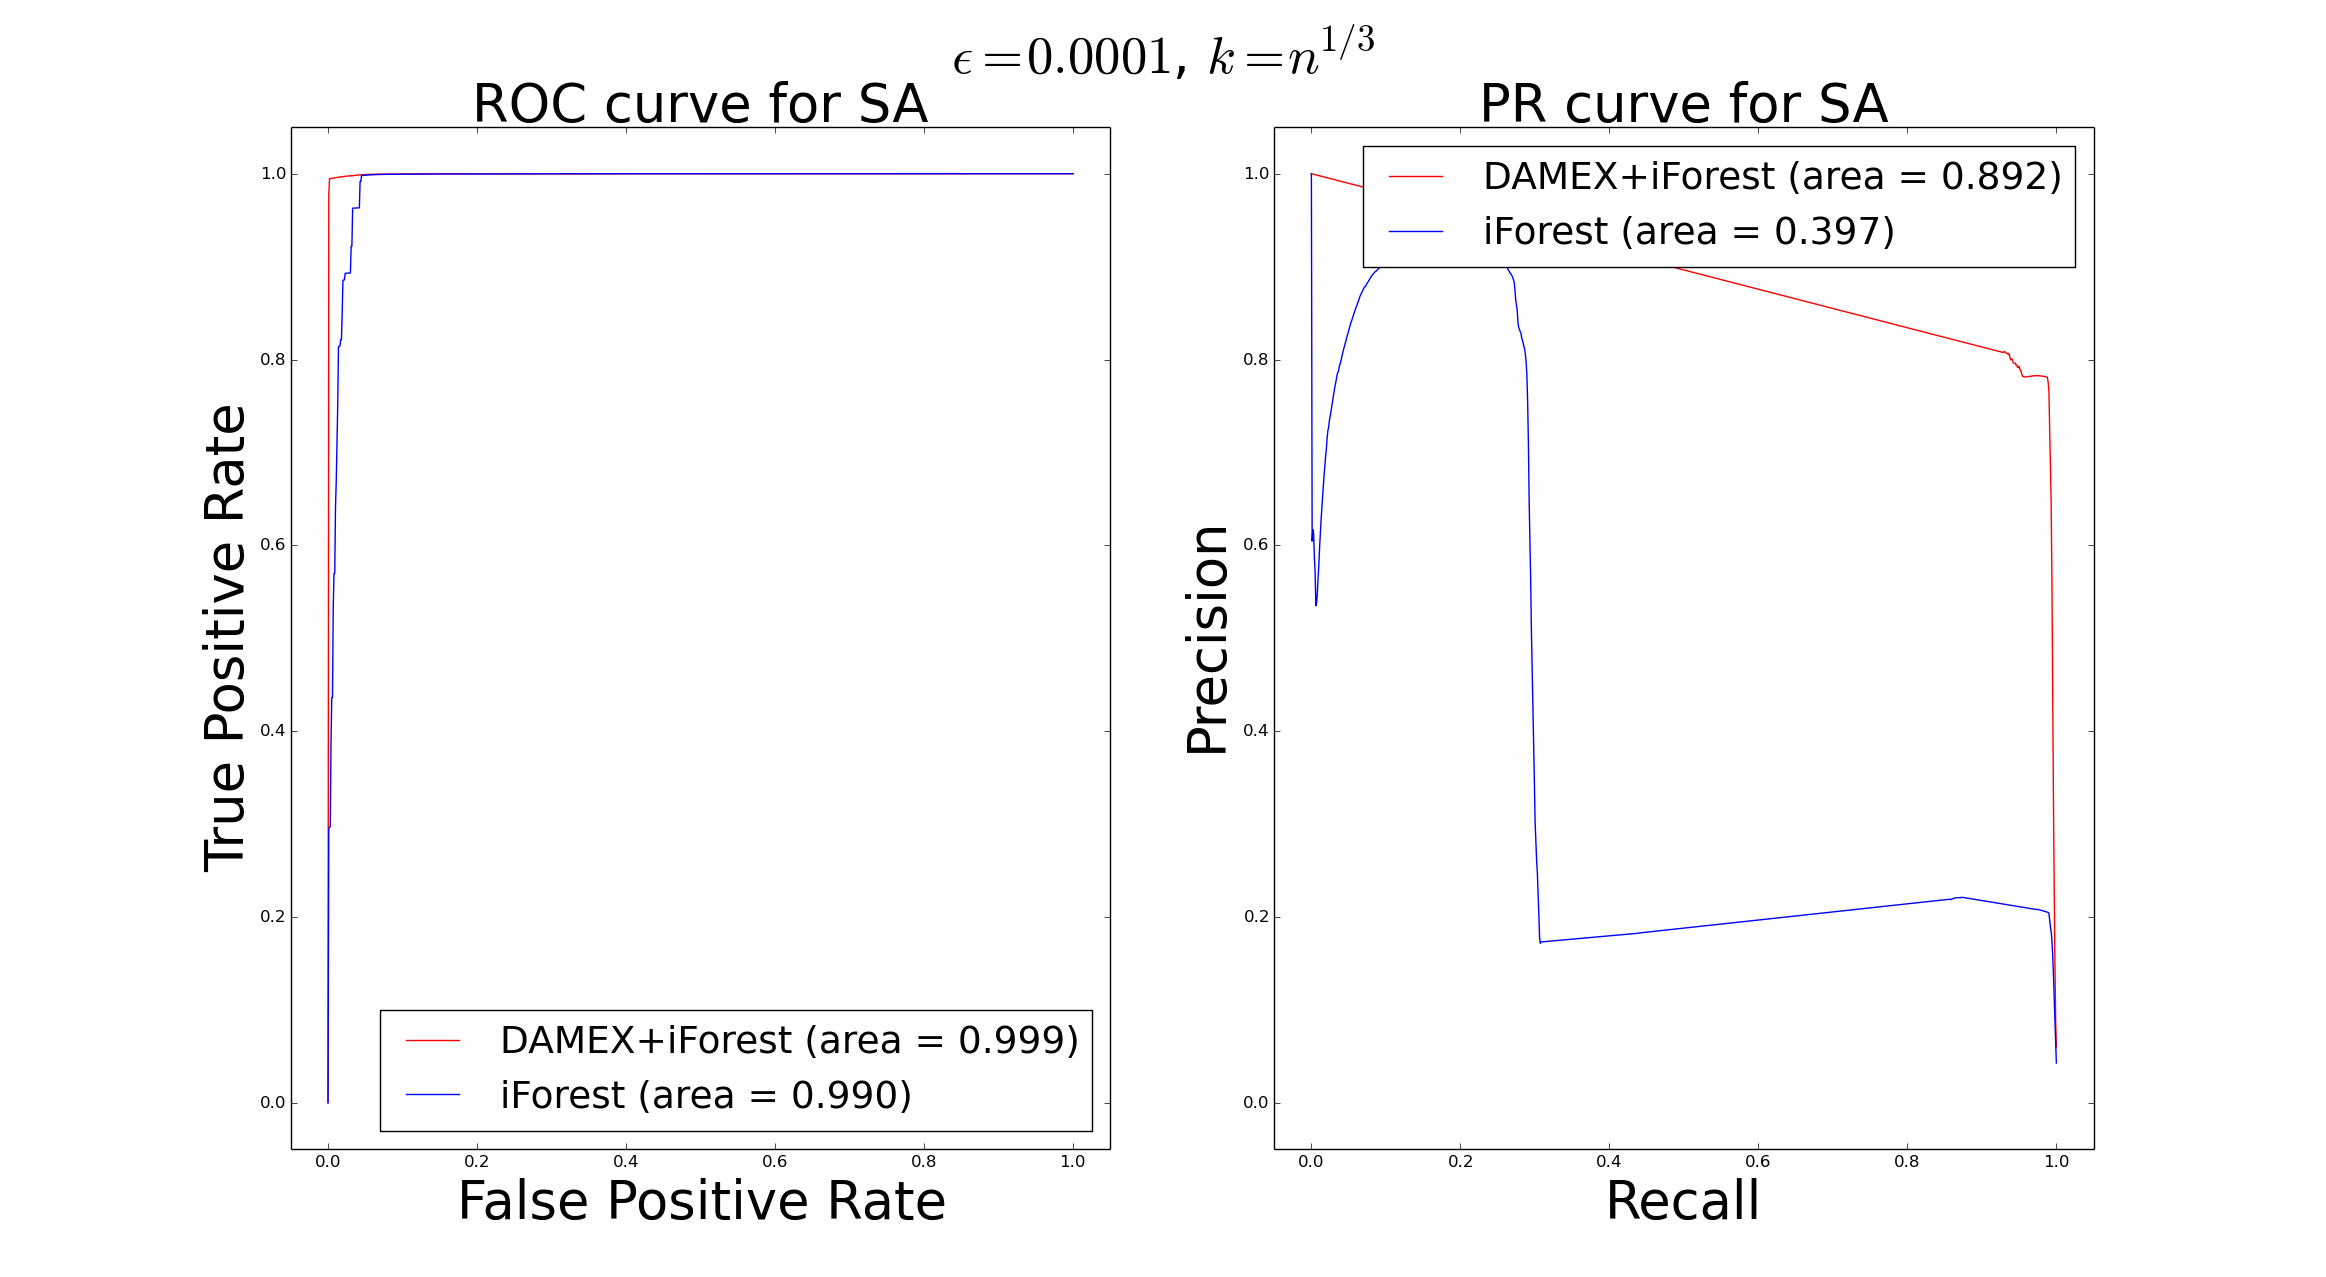
\includegraphics[width = 1. \textwidth]{sourcefigs/SA-lb-semi-supervised-average}
%   \caption{ROC and PR curve on SA dataset}
%   \label{SA}
% \end{figure}
% \end{frame}



% \begin{frame}
% \begin{figure}[ht]
%   \centering
%   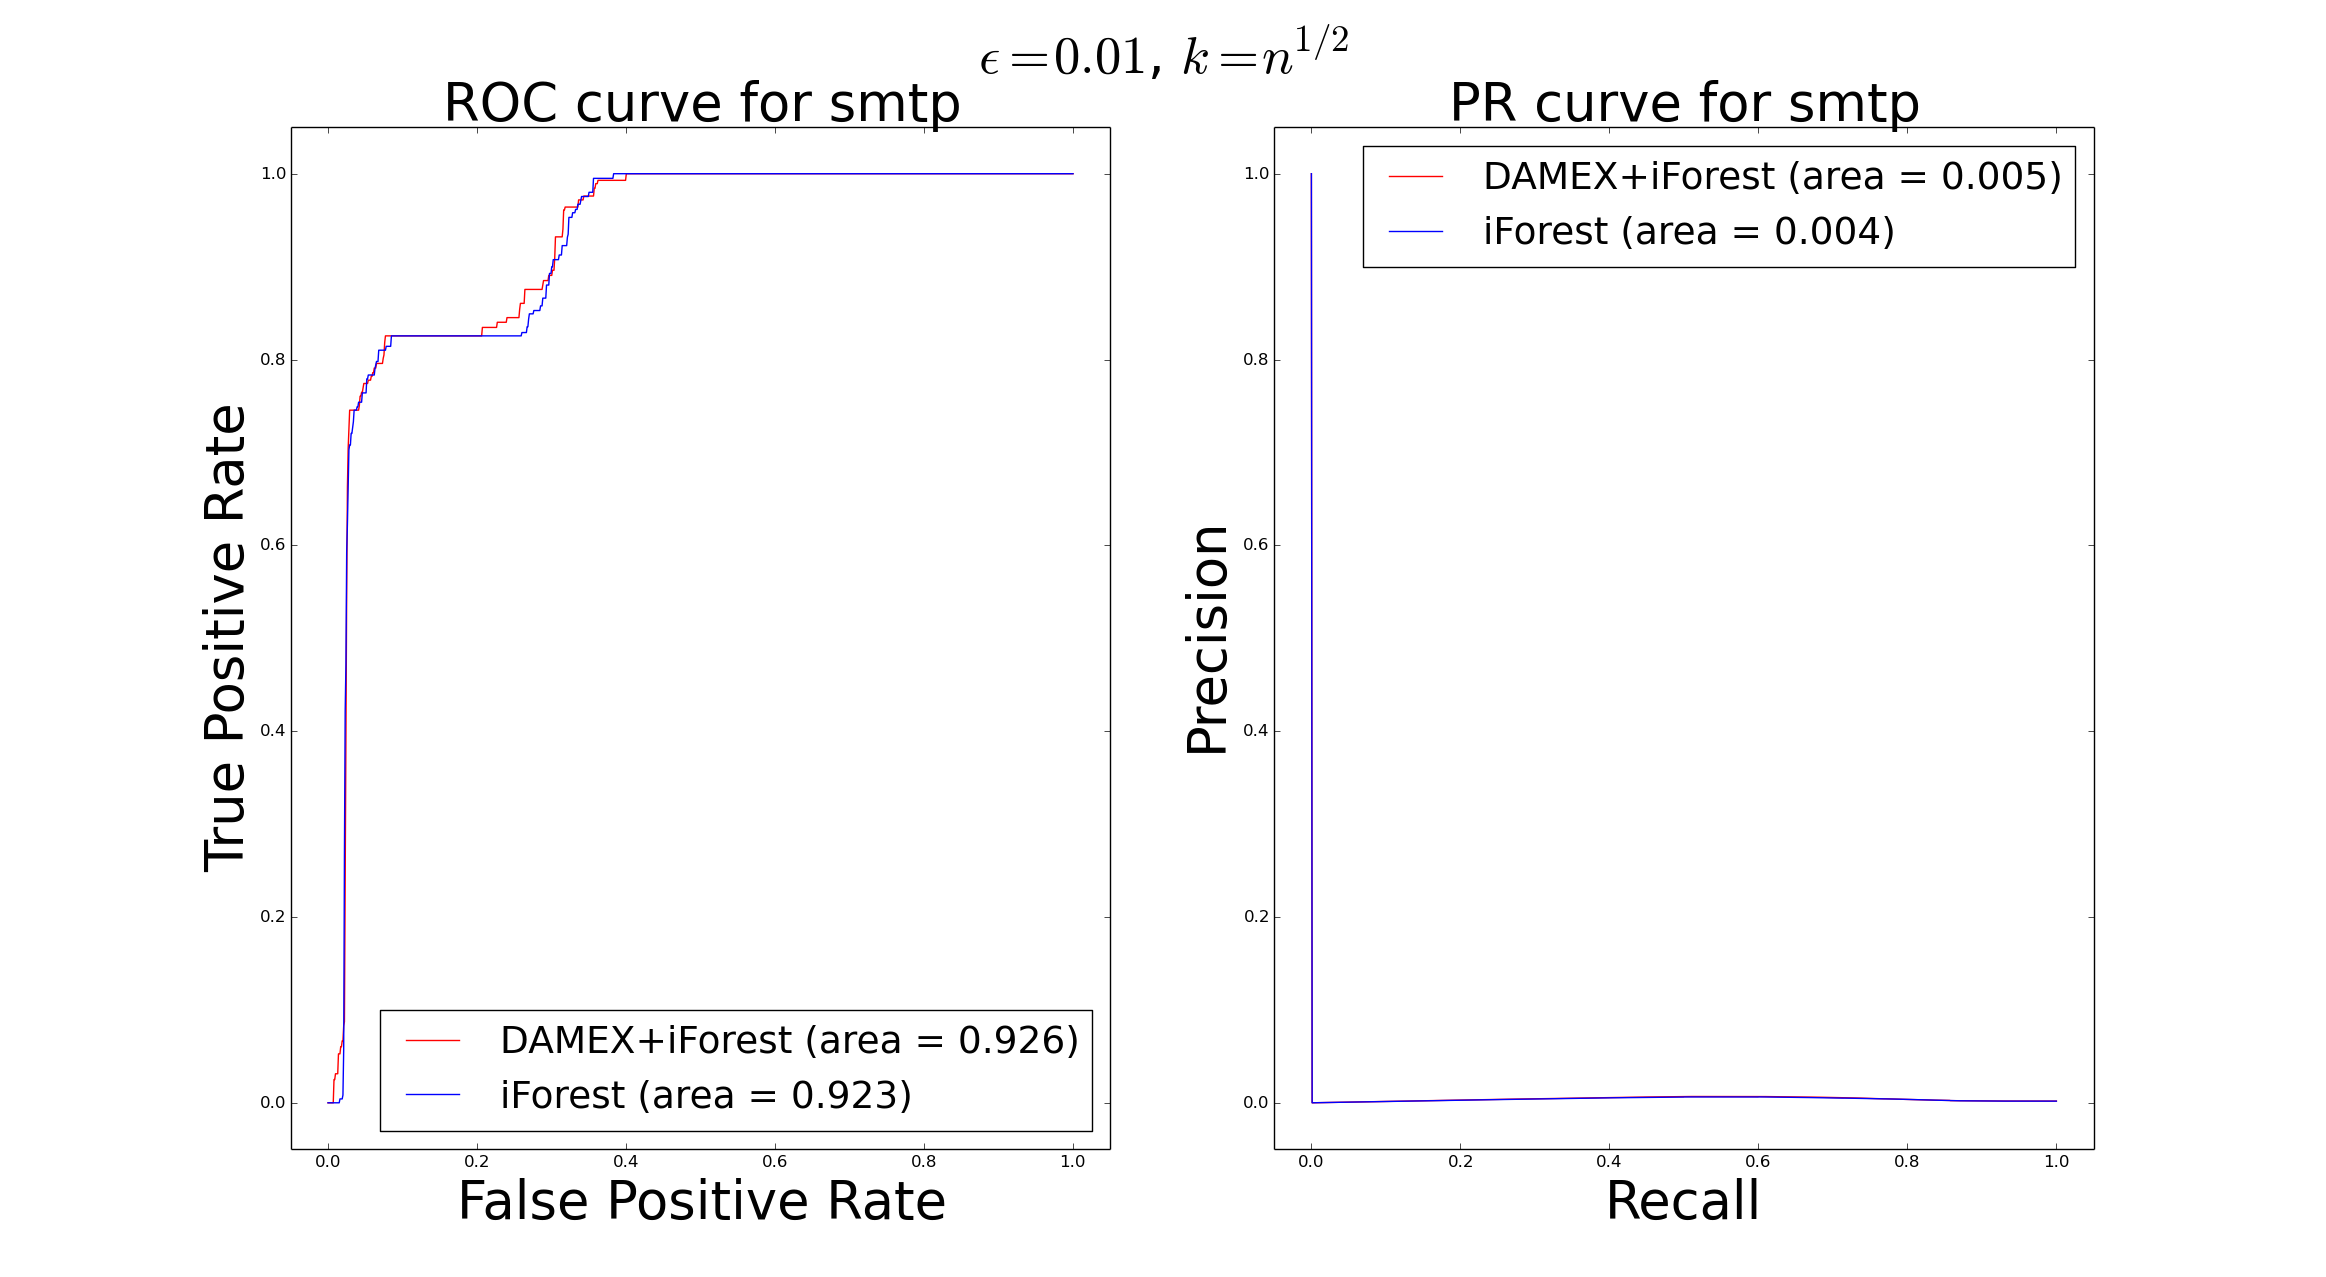
\includegraphics[width = 1. \textwidth]{sourcefigs/smtp-3d-semi-supervised-average}
%   \caption{ROC and PR curve on smtp dataset}
%   \label{smtp}
% \end{figure}
% \end{frame}













\begin{frame}
\centering
\Large{Thank you!}
\end{frame}



\begin{frame}
\frametitle{Benchmarks}
\begin{block}{Does performance in term of EM/MV correspond to performance in term of ROC/PR?}

\begin{itemize}
\item \textbf{Experiments:}
{\small
12 datasets, 3 AD algorithms (LOF, OCSVM, iForest)
$\to$ 36 possible pairwise comparisons:
\begin{align*}
\bigg\{~~\Big(A_1 \text{~on~} \mathcal{D},~ A_2 \text{~on~} \mathcal{D}\Big),~~ & A_1, A_2 \in \{\text{iForest, LOF, OCSVM}\}, \\
& \mathcal{D} \in \{\text{adult, http, \ldots, spambase}\} ~~\bigg\}.
\end{align*}
}


\item \textbf{Results:}
{ \small
If we only consider the pairs \st~\emph{ROC and PR agree on which algorithm is the best}, we are able (with EM and MV scores) to recover it in $80\%$ of the cases.
}
\end{itemize}


\end{block}
\end{frame}


\begin{frame}
\begin{table}[!ht]
\caption{Original Datasets characteristics}
\centering
%\tabcolsep=0.2cm
\resizebox{\linewidth}{!} {
\begin{tabular}{l cc ll }
  \toprule
  ~           & nb of samples      & nb of features     & ~~~~~~~~~~~~~~~~~~~~~~~~~anomaly class      & ~                  \\ \cmidrule{1-5}
  adult       & 48842              & 6                  &    class '$>50K$'                           &      (23.9\%)      \\
  http        & 567498             & 3                  &      attack                                 &    (0.39\%)        \\
  pima        & 768                & 8                  &    pos (class 1)                            &        (34.9\%)    \\
  smtp        & 95156              & 3                  &      attack                                 &    (0.03\%)        \\
  wilt        & 4839               & 5                  &    class 'w' (diseased trees)               &    (5.39\%)        \\
  annthyroid  & 7200               & 6                  &    classes $\neq$ 3                         &        (7.42\%)    \\
  arrhythmia  & 452                & 164                &    classes $\neq$ 1 (features 10-14 removed)&  (45.8\%)          \\
  forestcover & 286048             & 10                 &    class 4  (vs. class 2 )                  &           (0.96\%) \\
  ionosphere  & 351                & 32                 &    bad                                      &       (35.9\%)     \\
  pendigits   & 10992              & 16                 &    class 4                                  &        (10.4\%)    \\
  shuttle     & 85849              & 9                  &      classes $\neq$ 1 (class 4 removed)     &  (7.17\%)          \\
  spambase    & 4601               & 57                 &    spam                                     &           (39.4\%) \\
  \bottomrule
\end{tabular}
}
\end{table}

\end{frame}


\begin{frame}
\begin{table}[!ht]
\centering
\footnotesize
\caption{\footnotesize Results for the novelty detection setting. One can see that ROC, PR, EM, MV often do agree on which algorithm is the best (in bold), which algorithm is the worse (underlined) on some fixed datasets. When they do not agree, it is often because ROC and PR themselves do not, meaning that the ranking is not clear.}
\tabcolsep=0.11cm
\resizebox{\linewidth}{!} {
\begin{tabular}{l cccc c cccc c cccc}
\toprule
Dataset      & \multicolumn{4}{c}{iForest}& & \multicolumn{4}{c}{OCSVM}&  & \multicolumn{4}{c}{LOF} \\ %& parameters $(\epsilon, k)$\\
  \cmidrule{1-15}

~            & ROC  & PR   & EM    &  MV  &  & ROC  & PR   & EM    & MV     &  & ROC  & PR   & EM    & MV    \\
adult        &\bf 0.661 &\bf 0.277 &\bf 1.0e-04&\bf 7.5e01&  &0.642 &0.206 &2.9e-05& 4.3e02 &  &\underline{0.618} &\underline{0.187}&\underline{1.7e-05}&\underline{9.0e02} \\
http         &0.994 &0.192 &1.3e-03&9.0   &  &\bf 0.999 &\bf 0.970 &\bf 6.0e-03&\bf 2.6  &     &\underline{0.946} &\underline{0.035} &\underline{8.0e-05}&\underline{3.9e02} \\
pima         &0.727 &0.182 &5.0e-07&\bf 1.2e04&  &\bf 0.760 &\bf 0.229 &\bf 5.2e-07&\underline{1.3e04} &   &\underline{0.705} &\underline{0.155} &\underline{3.2e-07}&2.1e04 \\
smtp         &0.907 &\underline{0.005} &\underline{1.8e-04}&\underline{9.4e01}&  &\underline{0.852} &\bf 0.522 &\bf 1.2e-03&8.2    &   &\bf 0.922 &0.189 & 1.1e-03&\bf 5.8    \\
wilt         &0.491 &0.045 &4.7e-05&\underline{2.1e03} & &\underline{0.325} &\underline{0.037} &\bf 5.9e-05&\bf 4.5e02 &   &\bf 0.698 &\bf 0.088 &\underline{2.1e-05}&1.6e03 \\ 
 &&&&&&&&&&&&&& \\
% internet\_ads&0.414 &0.109 &  NA   &  NA    &      &      &       &          &0.540 &0.139 &       &       \\
% SA           &0.988 &0.386 &  NA   &  NA    &      &      &       &          &0.880 &0.018 &       &       \\
% SF           &0.936 &0.038 &  NA   &  NA    &      &      &       &          &0.891 &0.022 &       &       \\
annthyroid   &\bf 0.913 &\bf 0.456 &\bf 2.0e-04&2.6e02 & &\underline{0.699} &\underline{0.237} &\underline{6.3e-05}&\bf 2.2e02 &   &0.823 &0.432 &6.3e-05&\underline{1.5e03} \\
arrhythmia   &\bf 0.763 &\bf 0.487 &\bf 1.6e-04&\bf 9.4e01 & &0.736 &0.449 &1.1e-04&1.0e02   & &\underline{0.730} &\underline{0.413} &\underline{8.3e-05}&\underline{1.6e02} \\
forestcov.   &\underline{0.863} &\underline{0.046} &\underline{3.9e-05}&\underline{2.0e02}&  &0.958 &0.110 &5.2e-05&1.2e02  &  &\bf 0.990 &\bf 0.792 &\bf 3.5e-04&\bf 3.9e01 \\
ionosphere   &\underline{0.902} &\underline{0.529} &\underline{9.6e-05}&\underline{7.5e01} & &\bf 0.977 &\bf 0.898 &\bf 1.3e-04&\bf 5.4e01  &  &0.971 &0.895 &1.0e-04&7.0e01 \\
pendigits    &0.811 &0.197 &2.8e-04&2.6e01 & &\underline{0.606} &\underline{0.112} &\underline{2.7e-04}&\underline{2.7e01}   & &\bf 0.983 &\bf 0.829 &\bf 4.6e-04&\bf 1.7e01 \\
shuttle      &0.996 &0.973 &1.8e-05&5.7e03 & &\underline{0.992} &\underline{0.924} &\bf 3.2e-05&\bf 2.0e01   & &\bf 0.999 &\bf 0.994 &\underline{7.9e-06}&\underline{2.0e06} \\
spambase     &\bf 0.824 &\bf 0.371 &\bf 9.5e-04&\bf 4.5e01&  &\underline{0.729} &0.230 &4.9e-04&1.1e03  &  &0.754 &\underline{0.173} &\underline{2.2e-04}&\underline{4.1e04} \\
\bottomrule
\end{tabular}
}
\end{table}

\end{frame}

\end{document}
